%%%%%%%%%%%%%%%%%%%%%%%%%%%%%%%%%%%%%%%%%
% Thesis 
% LaTeX Template
% Version 1.3 (21/12/12)
%
% This template has been downloaded from:
% http://www.latextemplates.com
%
% Original authors:
% Steven Gunn 
% http://users.ecs.soton.ac.uk/srg/softwaretools/document/templates/
% and
% Sunil Patel
% http://www.sunilpatel.co.uk/thesis-template/
%
% License:
% CC BY-NC-SA 3.0 (http://creativecommons.org/licenses/by-nc-sa/3.0/)
%
% Note:
% Make sure to edit document variables in the Thesis.cls file
%
%%%%%%%%%%%%%%%%%%%%%%%%%%%%%%%%%%%%%%%%%

%----------------------------------------------------------------------------------------
%	PACKAGES AND OTHER DOCUMENT CONFIGURATIONS
%----------------------------------------------------------------------------------------

\documentclass[10pt, a4paper, oneside]{Thesis} % Paper size, default font size and one-sided paper

\graphicspath{{./Pictures/}} % Specifies the directory where pictures are stored
\hypersetup{urlcolor=blue, colorlinks=true} % Colors hyperlinks in blue - change to black if annoying
\title{\ttitle} % Defines the thesis title - don't touch this
\begin{document}

\frontmatter % Use roman page numbering style (i, ii, iii, iv...) for the pre-content pages

% Define the page headers using the FancyHdr package and set up for one-sided printing
\fancyhead{} % Clears all page headers and footers
\rhead{\thepage} % Sets the right side header to show the page number
\lhead{} % Clears the left side page header

\pagestyle{fancy} % Finally, use the "fancy" page style to implement the FancyHdr headers

\newcommand{\HRule}{\rule{\linewidth}{0.5mm}} % New command to make the lines in the title page

% PDF meta-data
\hypersetup{pdftitle={\ttitle}}
\hypersetup{pdfsubject=\subjectname}
\hypersetup{pdfauthor=\authornames}
\hypersetup{pdfkeywords=\keywordnames}

%----------------------------------------------------------------------------------------
%	TITLE PAGE
%----------------------------------------------------------------------------------------

\begin{titlepage}
\begin{center}

\textsc{\LARGE \univname}\\[1.5cm] % University name

\HRule \\[0.4cm] % Horizontal line
{\huge \bfseries \ttitle}\\[0.4cm] % Thesis title
\HRule \\[1.5cm] % Horizontal line
\begin{minipage}{0.8\textwidth} \Large
\centering
\emph{Author:}\\
\authornames
\end{minipage}\\[2cm]
 

\begin{minipage}{0.4\textwidth}
\centering
\emph{Supervisor:} \\
{\supname} 
\end{minipage}\\[3cm]

\begin{minipage}{0.4\textwidth}
\centering
\emph{Advisor:} \\
{\advname} 
\end{minipage}\\[3cm]
 

{\large HS15}\\[1cm] % Date

\includegraphics{eth_logo_kurz_pos.pdf} % University/department logo - uncomment to place it

\end{center}

\end{titlepage}

\setstretch{1.5}

\pagestyle{fancy} % The page style headers have been "empty" all this time, now use the "fancy" headers as defined before to bring them back

\lhead{\emph{Contents}} % Set the left side page header to "Contents"
\tableofcontents % Write out the Table of Contents

%----------------------------------------------------------------------------------------
%	CONTENT - CHAPTERS
%----------------------------------------------------------------------------------------

\mainmatter % Begin numeric (1,2,3...) page numbering

\pagestyle{fancy} % Return the page headers back to the "fancy" style

% Include the chapters of the thesis as separate files from the Chapters folder
% Uncomment the lines as you write the chapters

% Chapter Template

\chapter{Introduction and Motivation} % Main chapter title

\label{Introduction} % Change X to a consecutive number; for referencing this chapter elsewhere, use \ref{ChapterX}

\lhead{Chapter 1. \emph{Introduction}} % Change X to a consecutive number; this is for the header on each page - perhaps a shortened title

A number of projects aim to port \texttt{WaveBlocksND} (see \cite{waveblocksnd}) from a python implementation to a \texttt{C++} implementation. My task was the porting of the functionality responsible for handling matrix potentials and the Hagedorn propagator. In this report I will outline the desired functionality and elaborate on my design decisions leading to the current template-heavy implementation.

\section{Background}
\texttt{WaveBlocksND} is a python library to simulate the time-dependent behavior of semiclassical wavepackets on energy surfaces. These energy surfaces are described by matrix potentials $V$ : $\mathbb{R}^D \rightarrow \mathbb{R}^{N\times N}$. The simulation is advanced using a propagator which updates the parameters of a given wavepacket given $V$ and a timestep $dt$. One such propagator is the Hagedorn propagator (see \cite{FGL_semiclassical_dynamics}, \cite{H_ladder_operators}).
The following sections give a quick recapitulation of the relevant operations and properties required from these matrix potentials in \texttt{WaveBlocksND} (see \cite{B_master_thesis}).

\subsection{Matrix Potentials}
Consider matrix valued mappings from real space $\mathcal{C} : \mathbb{R}^D \rightarrow \mathbb{R}^{N\times N}$ \footnote{For certain set-ups it might be easier to consider complex matrix valued functions but the following statements can still be applied easily in that case as well.}. One can write these mappings in the form of a matrix parameterized with an $\mathbb{R}^D$ vector as follows:

\begin{equation}
\mathcal{C}(v) =  \begin{pmatrix}
  c_{1,1}(v) & c_{1,2}(v) & \cdots & c_{1,N}(v) \\
  c_{2,1}(v) & c_{2,2}(v) & \cdots & c_{2,N}(v) \\
  \vdots  & \vdots  & \ddots & \vdots  \\
  c_{N,1}(v) & c_{N,2}(v) & \cdots & c_{N,N}(v)
 \end{pmatrix}
 \label{eqn:matrixOfFunctions}
\end{equation}

where $c_{i,j} : \mathbb{R}^D \rightarrow \mathbb{R}$.

\subsection{Derivatives}
Using formulation \ref{eqn:matrixOfFunctions}, one can define the Jacobian of $\mathcal{C}$ as:
\begin{equation}
\begin{bmatrix}
  Dc_{1,1}(v) & Dc_{1,2}(v) & \cdots & Dc_{1,N}(v) \\
  Dc_{2,1}(v) & Dc_{2,2}(v) & \cdots & Dc_{2,N}(v) \\
  \vdots  & \vdots  & \ddots & \vdots  \\
  Dc_{N,1}(v) & Dc_{N,2}(v) & \cdots & Dc_{N,N}(v)
 \end{bmatrix}
 \label{eqn:matrixOfJacobians}
\end{equation}

where the use of the square brackets indicates that we are merely thinking of the matrix as a container rather than the mathematical object.

The Hessian of $\mathcal{C}$ can be defined accordingly.

\subsection{Quadratic Approximation}
The quadratic approximation $Q[f]: \mathbb{R}^D \rightarrow \mathbb{R}$ of a function $f: \mathbb{R}^D \rightarrow \mathbb{R}$ around some point $q \in \mathbb{R}^D$ is written as
\begin{equation}
Q[f](x) = f(q) + Df(q) \cdot (x-q) + {1 \over 2}(x-q)^T \cdot D^2f(q) \cdot (x-q)
\label{eqn:oneDimQuadratic}
\end{equation}

Similarly to the derivatives one can also express the element-wise quadratic approximation $Q[\mathcal{C}]$ of $\mathcal{C}$ as:
\begin{equation}
\begin{bmatrix}
  Q[c_{1,1}](v) & Q[c_{1,2}](v) & \cdots & Q[c_{1,N}](v) \\
  Q[c_{2,1}](v) & Q[c_{2,2}](v) & \cdots & Q[c_{2,N}](v) \\
  \vdots  & \vdots  & \ddots & \vdots  \\
  Q[c_{N,1}](v) & Q[c_{N,2}](v) & \cdots & Q[c_{N,N}](v)
 \end{bmatrix}
 \label{eqn:matrixOfQuadratics}
\end{equation}


\subsection{Eigenvalues}
While in principle, one can compute the eigenvalues and eigenvectors of $\mathcal{C}(x)$ point-wise as $\lambda_i(x)$ and $v_i(x)$ and then define the mapping
$\mathcal{D} : \mathbb{R}^D \rightarrow \mathbb{C}^{N\times N}$ as:
\begin{equation}
\mathcal{D}(x) = \begin{pmatrix}
  \lambda_1(x) & 0 & \cdots & 0 \\
  0& \lambda_2(x) & \cdots & 0 \\
  \vdots  & \vdots  & \ddots & \vdots  \\
  0 & 0 & \cdots & \lambda_N(x)
 \end{pmatrix}
 \label{eqn:diag}
\end{equation}

Furthermore, one can define the mapping $\mathcal{V} : \mathbb{R}^D \rightarrow \mathbb{C}^{N \times N}$ as:
\begin{equation}
\mathcal{V}(x) = \begin{pmatrix}
  v_1(x) & v_2(x) & \cdots & v_N(x)
 \end{pmatrix}
 \label{eqn:eigenTransform}
\end{equation}

one has to take care that the ordering of these \textit{eigenfunctions} does not change across evaluation points.
Since my implementation ignores this problem by forcing the user to provide the \textit{eigenfunctions} explicitly if he or she desires to use them, there is no need to go into further detail.

\subsubsection{Derivatives and Quadratic Remainder}
The derivatives and quadratic approximations are defined for $\mathcal{D}$ analogously to $\mathcal{C}$.

\subsection{Quadratic Remainder}
The quadratic remainder $R[f]: \mathbb{R}^D \rightarrow \mathbb{R}$ of a real valued function $f: \mathbb{R}^D \rightarrow \mathbb{R}$ around some point $q \in \mathbb{R}^D$ is simply defined as $R[f](x) = f(x) - Q[f](x)$.
However, the quadratic remainder of a matrix potential $\mathcal{C}$ is not defined point-wise for the purposes of \texttt{WaveBlocksND} but as follows (see \cite{B_master_thesis}):

\begin{equation}
R[\mathcal{C}](x) = \mathcal{C}(x) - Q[\mathcal{L}(x)]
\label{eqn:quadRemainder}
\end{equation}
where either $\mathcal{L}(x) = \lambda_\chi(x)I$ for some \textit{leading level} $\chi$ or in the homogeneous case or $\mathcal{L} = \mathcal{D}$.



% Chapter Template

\chapter{Programming Techniques} % Main chapter title

\label{progtech} % Change X to a consecutive number; for referencing this chapter elsewhere, use \ref{ChapterX}

\lhead{Chapter 2. \emph{Programming Techniques}} % Change X to a consecutive number; this is for the header on each page - perhaps a shortened title

In this chapter, I outline some programming techniques and the issues tackled with them during the design of the code.
%----------------------------------------------------------------------------------------
%	SECTION 1
%----------------------------------------------------------------------------------------
\section{A static approach to abstract base classes}
In this section, I quickly outline a common technique to obtain some of the functionality that virtual function calls provide without incurring the runtime costs associated with such calls.

\subsection{Curiously recurring template pattern (CRTP)}
CRTP (term coined in \cite{C_CRTP}) is a template pattern where a class template \texttt{B} expecting a class as parameter exists and next a class \texttt{D} is defined to inherit from an instantiation of \texttt{B} with the subtype \texttt{D} as argument.

\begin{lstlisting}[language=C++]
template<class Subtype>
struct Base {};

struct Derived : Base<Derived> {};
\end{lstlisting}

\subsection{Static Polymorphism}
Static polymorphism\footnote{See for example the Wikipedia article \url{https://en.wikipedia.org/wiki/Template_metaprogramming\#Static_polymorphism}} is an attempt to simulate some behavior of dynamic polymorphism (such as virtual functions) without the run-time costs associated. To achieve this one can make use of the CRTP. 

\begin{minipage}{\linewidth}
\begin{lstlisting}[language=C++]
template<class Subtype>
struct Base {
	int foo(int x) {
    	return static_cast<Subtype*>(this)->foo_implementation(x);
    }
    int bar(int x) {
    	return foo(x)+1;
    }
};

struct Derived : Base<Derived> {
	int foo_implementation(int x) { return x;}
};

struct OtherDerived : Base<OtherDerived> {
	int foo_implementation(int x) { return 2*x;}
};
\end{lstlisting}
\end{minipage}


In the example above we can see that there now is an interface \texttt{Base} indicating which functions are available and two implementations \texttt{Derived} and \texttt{OtherDerived} which implement the interface in different manners.
Note that \texttt{Derived} and \texttt{OtherDerived} are not subtypes of the same class as each template instantiation defines its own base class. We therefore lose the flexibility of choosing the implementation at runtime but gain the speed-up of statically linking to the implementation.

This really becomes useful when we want an abstract base class to provide some general functionality and then introduce specializations without the cost of having virtual function calls. 

In the above example both implementations inherit the common functionality \texttt{bar} from their respective base class while defining their own implementation of \texttt{foo}.

\section{Multiple Inheritance and Linearization}
\texttt{C++} allows a class to inherit from multiple base classes. While this means that we can easily combine implementations it is not without disadvantages. In this section, I wish to outline a commonly occuring issue with multiple inheritance, possible solutions thereof and finally the application of one of these solutions to my implementation.\footnote{The elaborations in this section are largely based on  Chapters "Multiple Inheritance" and "Linearization" of the  lecture "Concepts of Object Oriented Programming" by Prof. Peter M\"uller. See the lecture notes at \url{https://www1.ethz.ch/pminf/education/courses/coop}.} I particularly wish to discuss a problem arising from diamond shaped inheritance.
\subsection{Problem}
\begin{minipage}{\linewidth}
\begin{lstlisting}[language=C++]
struct A {
    virtual int bar(int x) {
    	return x+1;
    }
};

class B1 : public A {
};

class B2 : public A {
};

class C : public B1, public B2 {
	int foo() {
		return bar(2); // Which bar?
    }
};
\end{lstlisting}
\end{minipage}
An ambiguity arises with multiple inheritance whenever two or more of the base classes share a base class. In the example above, one has to explicitly select either \texttt{B1::bar} or \texttt{B2::bar} in the example above. Alternatively, one can  make the inheritance from \texttt{A} \texttt{virtual}. While this isn't without issue itself (especially since it requires foresight from the writers of \texttt{B1} and \texttt{B2} to inherit only virtually), my main concern here was the virtual inheritance itself since I wanted to avoid runtime penalties at all costs.

\subsection{Solution}
A common trick is to simply template the middle classes on their super class and forcing the writer of the child class \texttt{C} to choose the linearization order when inheriting\footnote{This somewhat emulates the linearization of traits as in Scala.}. While \texttt{B1} and \texttt{B2} can now inherit from \texttt{A} it is also possible to linearize the diamond shaped inheritance to single inheritance. While this solution certainly isn't without issues of its own\footnote{See again Prof. Peter M\"uller's lecture "Concepts of Object Oriented Programming" and its discussion of Scala traits as an example.}, I found it quite useful.

\begin{minipage}{\linewidth}
\begin{lstlisting}[language=C++]
struct A {
    virtual int bar(int x) {
    	return x+1;
    }
};

template<class Super>
class B1 : public Super {
};

template<class Super>
class B2 : public Super {
};

class C : public B1<B2<A>> {
	int foo() {
		return bar(2); // Which bar? Last override!
    }
};
\end{lstlisting}
\end{minipage}

\subsection{Application}
I make use of multiple inheritance to create a collection of modules which can be mixed and matched to provide only the functionality required to the class. To avoid diamond shaped inheritance every implementation that needs to inherit from some other implementation is templated on its super class. As an example of the mixing of modules consider a user that wants to create a potential only to evaluate it in some points and a user that wishes to also evaluate the derivatives. Both can make use of the same implementation for evaluation which requires both users to specify the potential. However, only the user that wishes to mix in (via inheritance) the functionality to also evaluate the derivatives is required to provide these during construction. This allows the users to easily create classes which only require and offer the functionality they desire. 

\section{Partial specializations}
\texttt{C++} does not allow partial specialization of template functions. It does, however, allow partial specialization of template classes. Therefore, a well known trick is to use a static member function of a template class, to effectively emulate partial specializations of functions.

\begin{minipage}{\textwidth}
\begin{lstlisting}[language=C++]
template<int N, int D>
int bar() {return 0;}

template<int N>
int bar<N,1>(){return 1;} // not allowed

template<int N, int D>
struct A {
	static int foo(){return 0;}
};

template<int N>
struct A<N,1> {
	static int foo(){return 1;} // allowed
};

int main() {
	A<2,2>::foo(); // 0
	A<2,1>::foo(); // 1
}
\end{lstlisting}
\end{minipage}

\section{Template specialization and template aliases}
During the coding I came across one strange issue related to template aliases which stumped me so much that I had to resort to asking a question on \url{stackoverflow.com}\footnote{The following description of the issue is very similar to the one I submitted to \url{http://stackoverflow.com/questions/32723988/alias-of-class-template} and the explanation of the issue is adapted from the accepted answer \url{http://stackoverflow.com/a/32724096/3139931} by user 'Barry'.}.

Consider an alias template \texttt{A}. Now let \texttt{B} be an alias template of \texttt{A}.
In the code below these class templates are used as template arguments for a struct \texttt{C} which is only specialized for one of the templates (\texttt{A}). \texttt{clang -std=c++11} exits with \texttt{error: implicit instantiation of undefined template 'C<B>'} indicating that another specialization for \texttt{B} is needed.
\begin{lstlisting}[language=C++]
template<int N>
using A = int;

template<int N>
using B = A<N>;

template<template<int> class I>
struct C;

template<>
struct C<A> {};

int main() {
  C<A> c;
  C<B> d; // clang error: implicit instantiation
}
\end{lstlisting}
It is strange that - despite not allowing specializations of aliases and therefore guaranteeing that both aliases will \textit{behave} the same - \texttt{A} and \texttt{B} are treated as different class templates because the standard only guarantees that \texttt{A<X>} and \texttt{B<X>} are the same for every class \texttt{X}. Logically we should then be able to assume that \texttt{A} and \texttt{B} are in fact the same since they behave exactly the same but there are no guarantees from the standard (and \texttt{clang} for example does treat them as two different templates). This is CWG issue \#1286\footnote{\url{http://www.open-std.org/jtc1/sc22/wg21/docs/cwg_active.html\#1286}}

Concretely, this problem means that we initially could not use an alias template for the really wordy typenames \texttt{matrixPotentials::bases::Canonical} and \texttt{matrixPotentials::bases::Eigen} since some implementations used to be specialized on those templates and would not have been guaranteed to be specialized on an alias template of these typenames. To spare the user from typing this wordy symbol one could either move them out of their nested namespaces, resort to using a macro or refactor the code to remove any templates specialized on a template themselves. I opted for the refactoring. Unfortunately, this issue does now restrict any future implementations from specializing on these basis templates.



% Chapter Template

\chapter{Code} % Main chapter title

\label{Code} % Change X to a consecutive number; for referencing this chapter elsewhere, use \ref{ChapterX}

\lhead{Chapter 3. \emph{Code}} % Change X to a consecutive number; this is for the header on each page - perhaps a shortened title

%----------------------------------------------------------------------------------------
%	SECTION 1
%----------------------------------------------------------------------------------------

\section{Libraries}
The implementation relies heavily on the \texttt{Eigen}\cite{eigenweb} template library for linear algebra. I have introduced a handful of template aliases to simplify the typenames of the most commonly used objects. Additionally, the code utilizes \texttt{eigen3-hdf5}\cite{eigen3-hdf5} for the serialization of the \texttt{Eigen} matrices into \texttt{hdf5} files.

\section{Matrix Potential}
In this section, I list all of the modules that can be used to create a matrix potential and elaborate on how to combine them.

\subsection{Abstract and Standard Implementation}
Most modules contain a class called \texttt{Abstract} which defines the functionality the module offers and implements some common functionality. This is usually the extension of an evaluation from a single point to a grid of points. Each module then provides at least one implementation (if only one implementation is provided, it is called \texttt{Standard}) of \texttt{Abstract} which inherits from \texttt{Abstract} using static polymorphism as described in the previous chapter. To add his or her own implementations the user can simply follow the pattern of the standard implementation. As an example, a user could define his or her own implementation of the \texttt{taylor} module wherein all of the evaluations are hard-coded instead of delegated to lambda functions for a more efficient evaluation.

\subsection{Namespaces}
To keep the global namespace and the \texttt{waveblocks} namespace unpolluted with implementation details all matrix potential related implementations are put within their own namespace \texttt{matrixPotentials} which contains a namespace \texttt{modules} which in turn contains a namespace for each module. Only standard implementations are exported via template aliases.

\subsubsection{Bases}
The \texttt{bases} namespace contains the class templates for the basis classes \texttt{Canonical} and \texttt{Eigen}. These are merely a collection of constants and aliases to make templating easier. Instead of a module depending on a large number of types it simply depends on a \textit{basis} and imports the required types via a macro.
\texttt{Canonical} and \texttt{Eigen} are exported to the \texttt{waveblocks} namespace via template aliases.

\subsubsection{Potentials}
The \texttt{potentials} namespace contains template aliases for often used configurations of modules such as a scalar valued potential which supports evaluation of the local quadratic remainder.

\subsubsection{Modules}
\begin{itemize}
\item \texttt{evaluation}: allows to evaluate a potential in one or many points
\item \texttt{jacobian}: allows to evaluate the Jacobian as defined in Chapter \ref{Introduction} in one or many points
\item \texttt{hessian}: allows to evaluate the Hessian as defined in Chapter \ref{Introduction} in one or many points
\item \texttt{exponential}: allows to evaluate the exponential of the resulting matrix of an evaluation in one or many points
\item \texttt{taylor}: allows to evaluate the potential, Jacobian and Hessian all at once in one or many points
\item \texttt{localQuadratic}: allows to evaluate the local quadratic of a matrix potential as defined in Chapter \ref{Introduction}
\item \texttt{leadingLevelOwner}: allows to define a potential which owns another potential
\item \texttt{localRemainder}: allows to define a potential whose local quadratic remainder can be computed as defined in Chapter \ref{Introduction}
\end{itemize}

\paragraph{Standard Implementations}
Figure \ref{fig:dia} shows the class diagram of the standard implementations of the modules available. Note that this class diagram only holds when using the template aliases provided by each module (i.e. using \texttt{waveblocks::Evaluation} rather than \texttt{waveblocks::matrixPotentials::modules::evaluation::Standard} as the standard implementations are usually more general and allow passing the super class as a template argument in most cases.
\begin{figure}
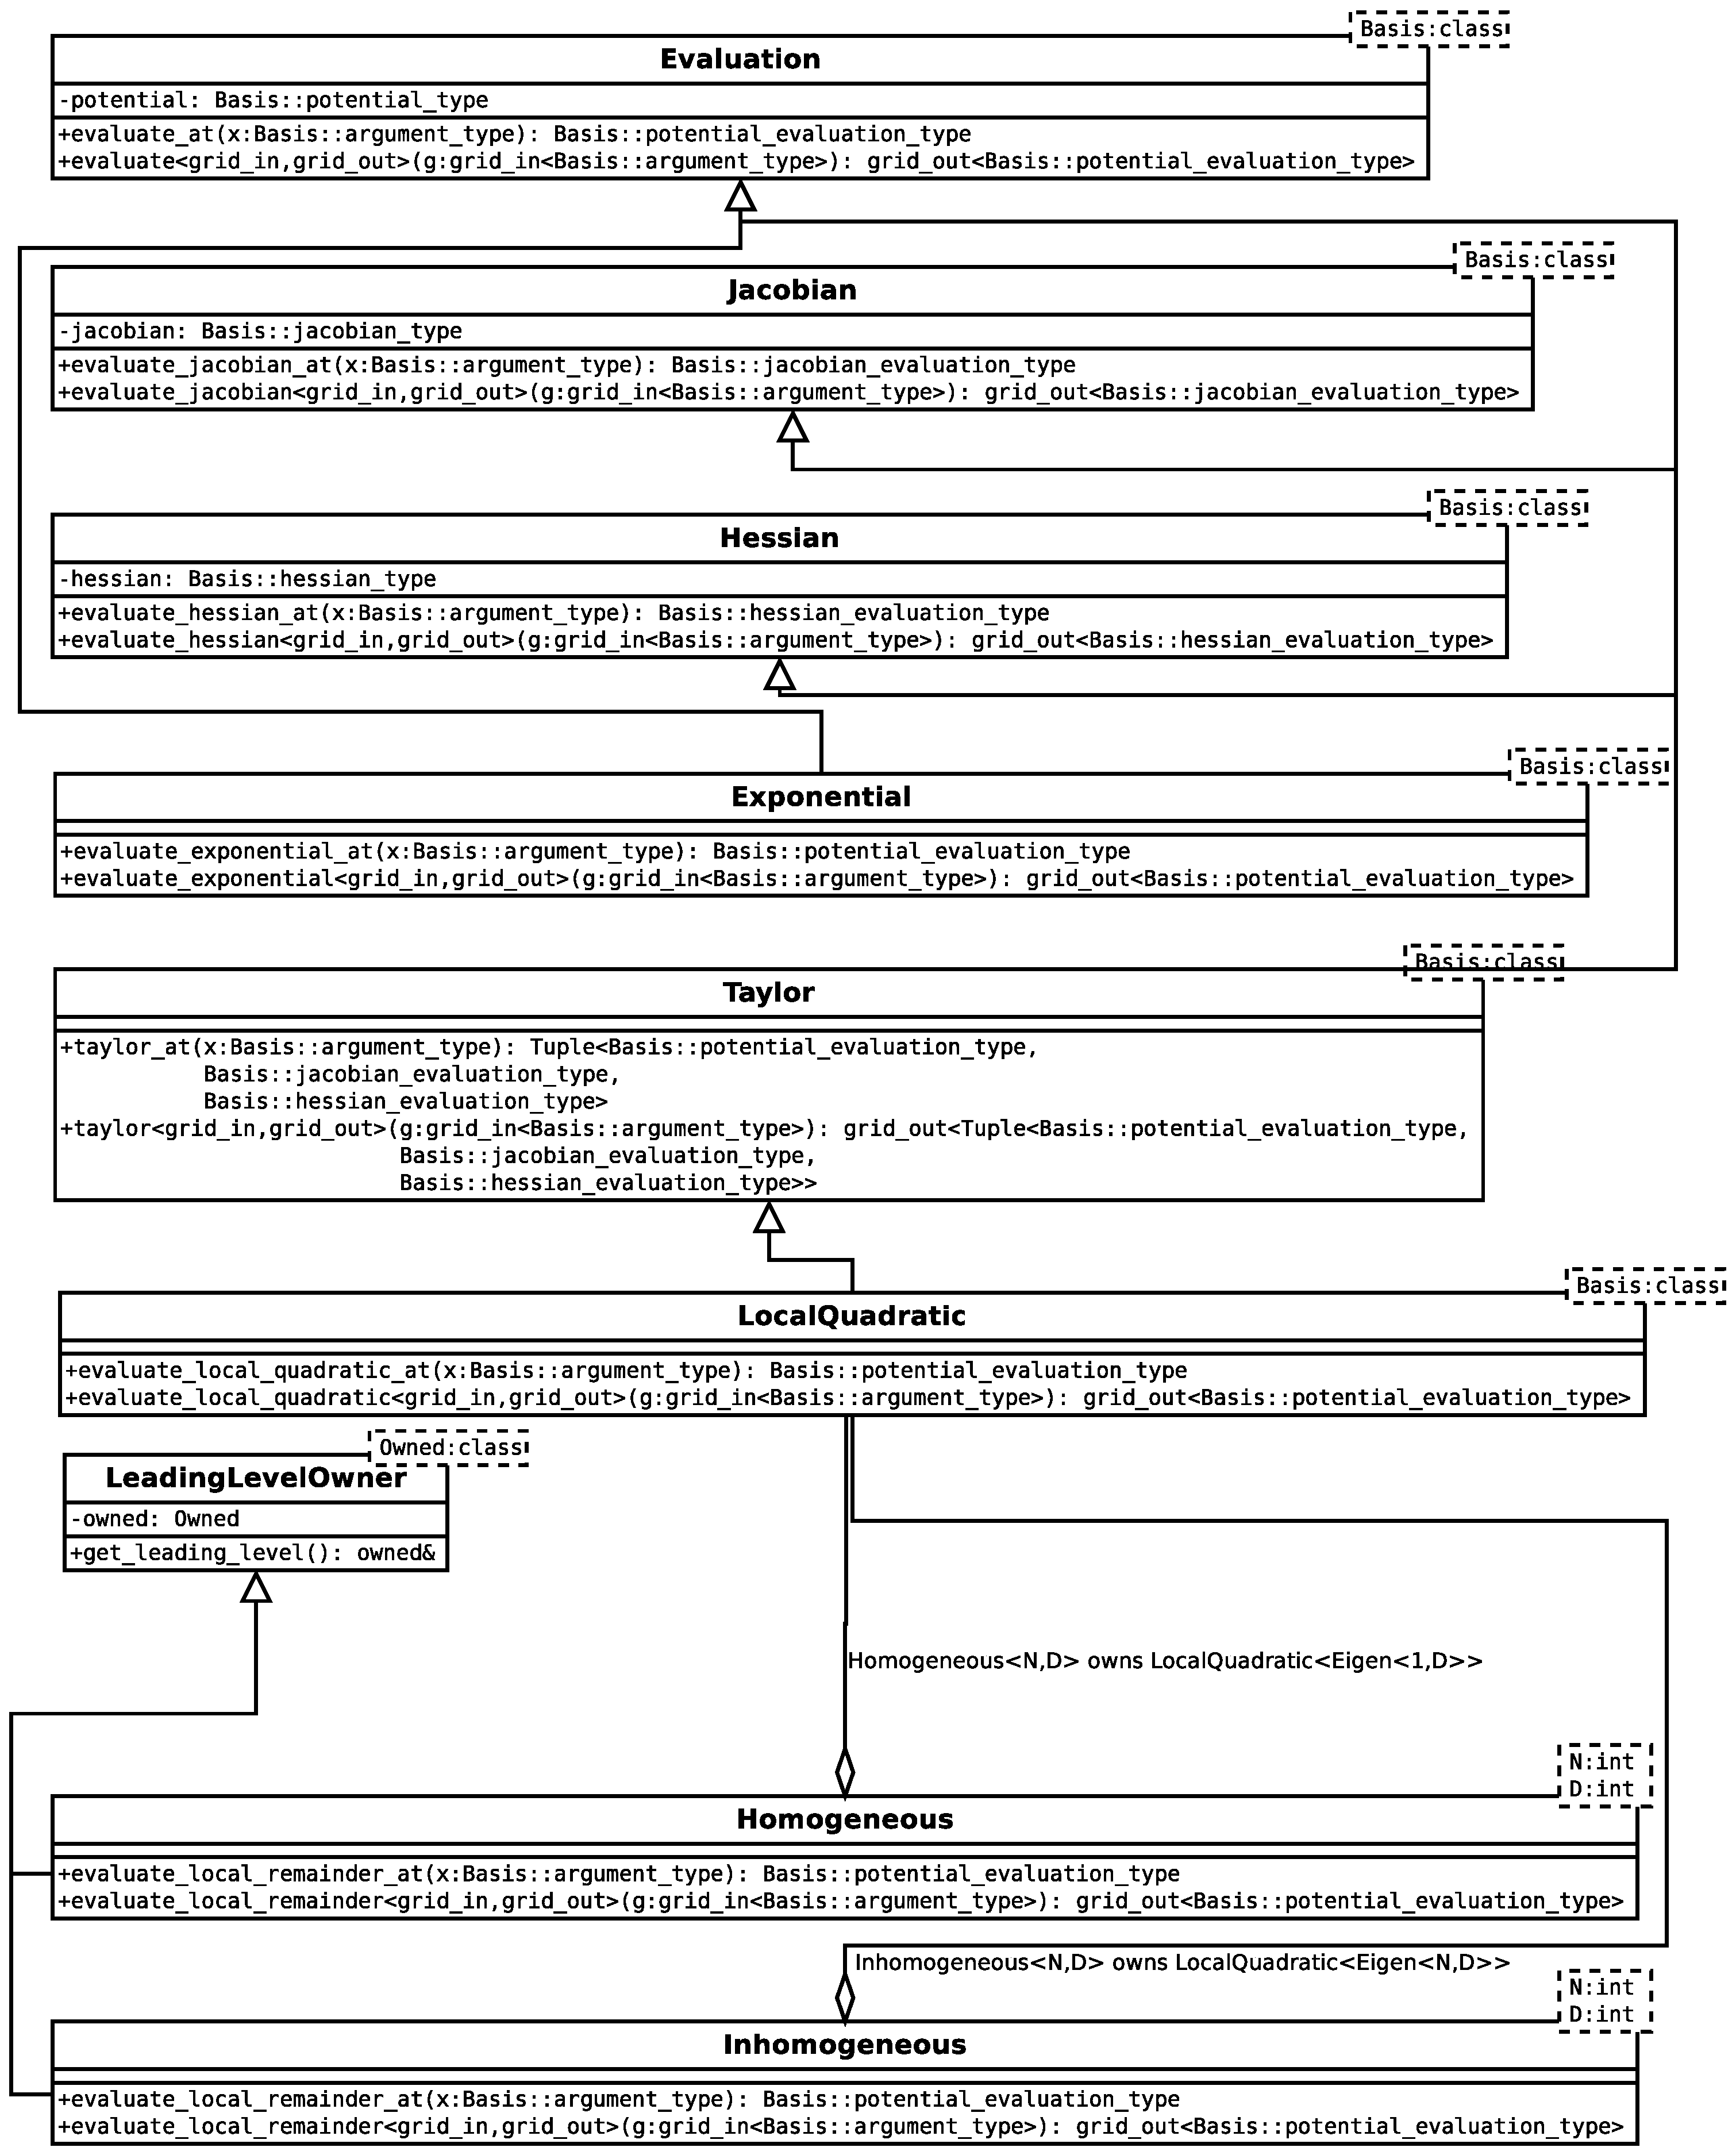
\includegraphics[width=\textwidth]{Figures/standardModules.eps}
\caption{Diagram of the standard implementations of the modules available and their class hierarchy. All of these classes are available in the \texttt{waveblocks} namespace.}
\label{fig:dia}
\end{figure}
\section{Hagedorn Propagator}
The Hagedorn propagator is implemented as a template class templated on the number of levels $N$, the dimension $D$, as well as the class \texttt{MultiIndex}, used for indexing the wavepacket, and the class \texttt{TQR}, which defines the tensor quadrature rule.
It offers the static method propagate which is overloaded for homogeneous and inhomogeneous wavepackets and specialized for scalar wavepackets. 
The propagator needs different implementations for $N=1$, $N>1$, $D=1$, $D>1$ as well as different implementations for homogeneous and inhomogeneous wavepackets. However, there exists a lot of overlap in these implementations which I make heavy use of by delegating non-overlapping parts to partially specialized template functions. As an example we can see that for the first step the inhomogeneous case simply iterates over all components and applies the same operation to the parameter set of the Hagedorn wavepacket propagated as the homogeneous case does. Similarly, there are only a few lines of code that need to be adjusted when dealing with $D=1$.

 
% Chapter Template

\chapter{Simulations} % Main chapter title

\label{Chapter4} % Change X to a consecutive number; for referencing this chapter elsewhere, use \ref{ChapterX}

\lhead{Chapter 4. \emph{Simulation}} % Change X to a consecutive number; this is for the header on each page - perhaps a shortened title

%----------------------------------------------------------------------------------------
%	SECTION 1
%----------------------------------------------------------------------------------------

\section{Verification}
To verify the implementation, I applied it to a 2D harmonic oscillator as well as a 1D anharmonic oscillator and compared the results to the results obtained with \texttt{WaveBlocksND}.
The computation attempts to find solutions to the time-dependent Schr\"odinger equation in
the semi-classical scaling:
\begin{equation}
i \varepsilon \frac{\partial}{\partial t}\Psi(\mathbf{x},t) = H \Psi(\mathbf{x},t)
\end{equation}
where $H = T + V$ and $T = -\sum\limits_{j=1}^D \varepsilon^2 \frac{\partial^2}{\partial \mathbf{x}^2_j}$ and $V$ is a potential.

\subsection{Harmonic Oscillator}
Consider a 2D harmonic potential.
A Gaussian Hagedorn wavepacket with $5$ cubic shape basis functions with the following initial parameters:
\begin{center}
 \begin{tabular}{|c c c c c c|} 
 \hline
 q & p & Q & P & S & $\varepsilon$\\ [0.5ex] 
 \hline
 $\begin{pmatrix}
 -3\\
 0\\
 \end{pmatrix}$ & $\begin{pmatrix} 0 \\ 0.5 \end{pmatrix}$ & I & iI & 0 & 0.1\\ 
 \hline
\end{tabular}
\end{center}
is propagated using the Hagedorn propagator with $dt = 0.01$ up to $T = 12$.


In Figures \ref{fig:harmonic_energy}, \ref{fig:harmonic_drift}, \ref{fig:harmonic_params} and \ref{fig:harmonic_coeffs} one observes conservation of energy and periodic behavior in the parameters of the wavepacket as well as constant coefficients, which is as expected since the local remainder must be zero. These results align neatly with the ones computed by \texttt{WaveBlocksND} giving confidence that at least the harmonic part of the implementation in the higher dimensional case is correct.
\begin{figure}[!th]
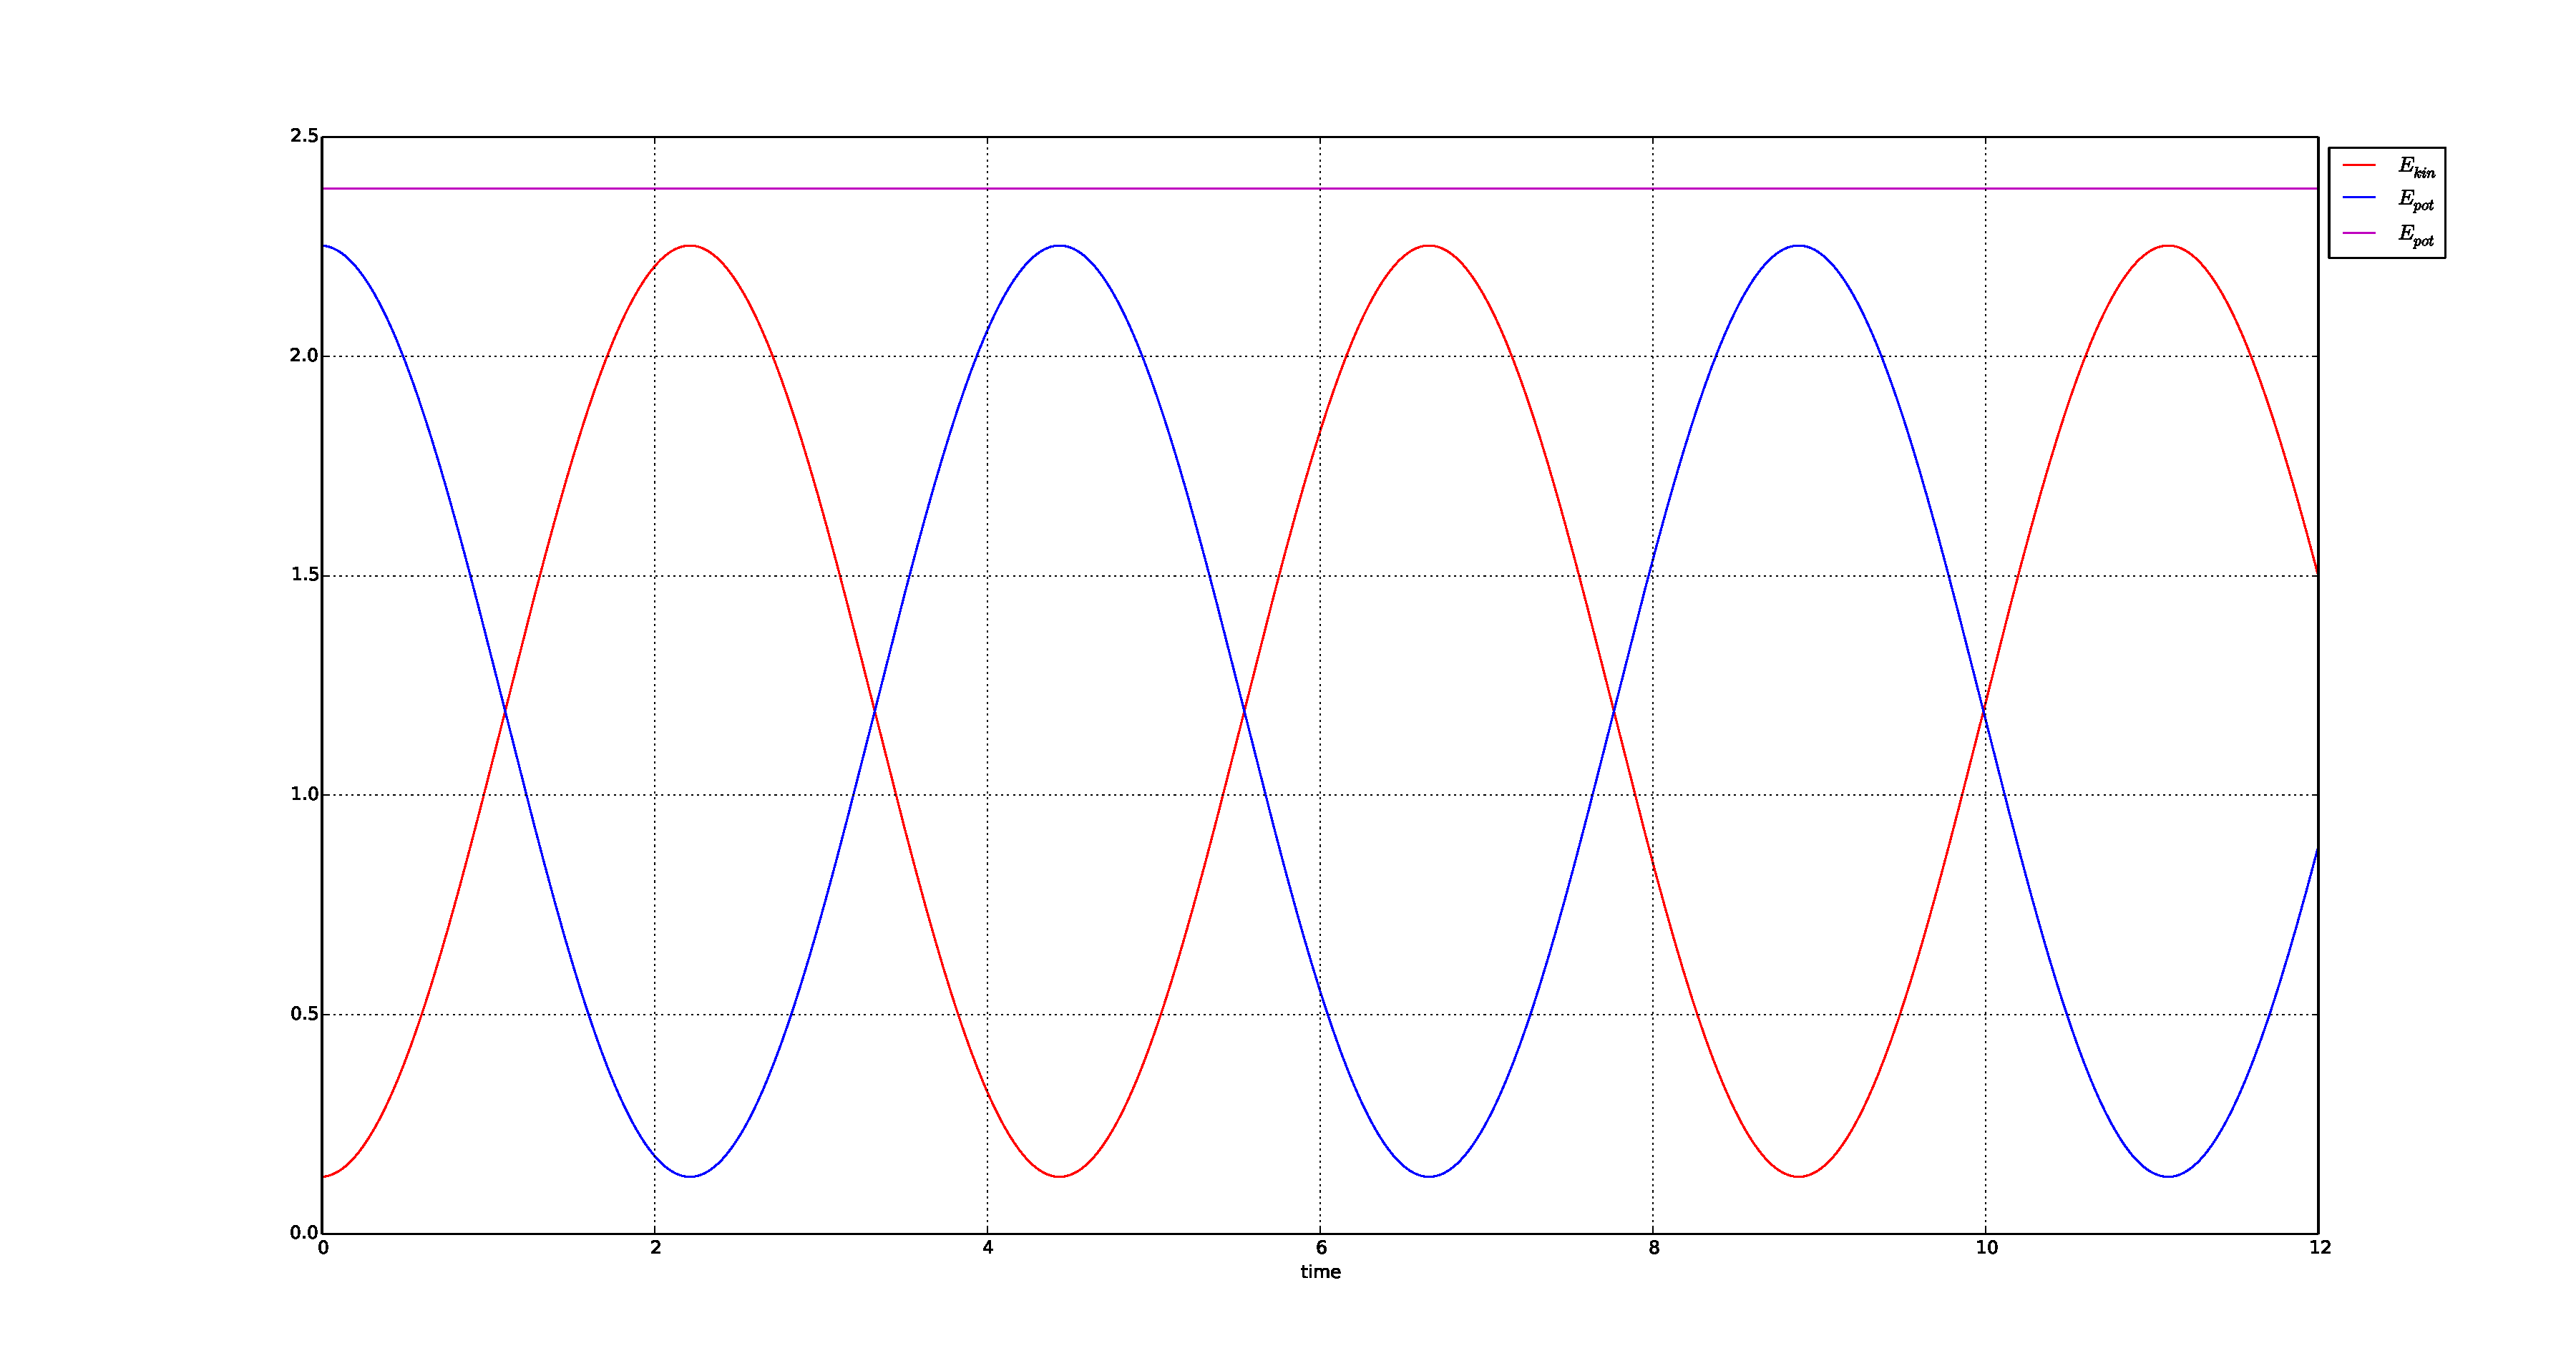
\includegraphics[width=\textwidth]{Figures/harmonic_energy.pdf}
\caption{The energies of the harmonic simulation.}
\label{fig:harmonic_energy}
\end{figure}

\begin{figure}
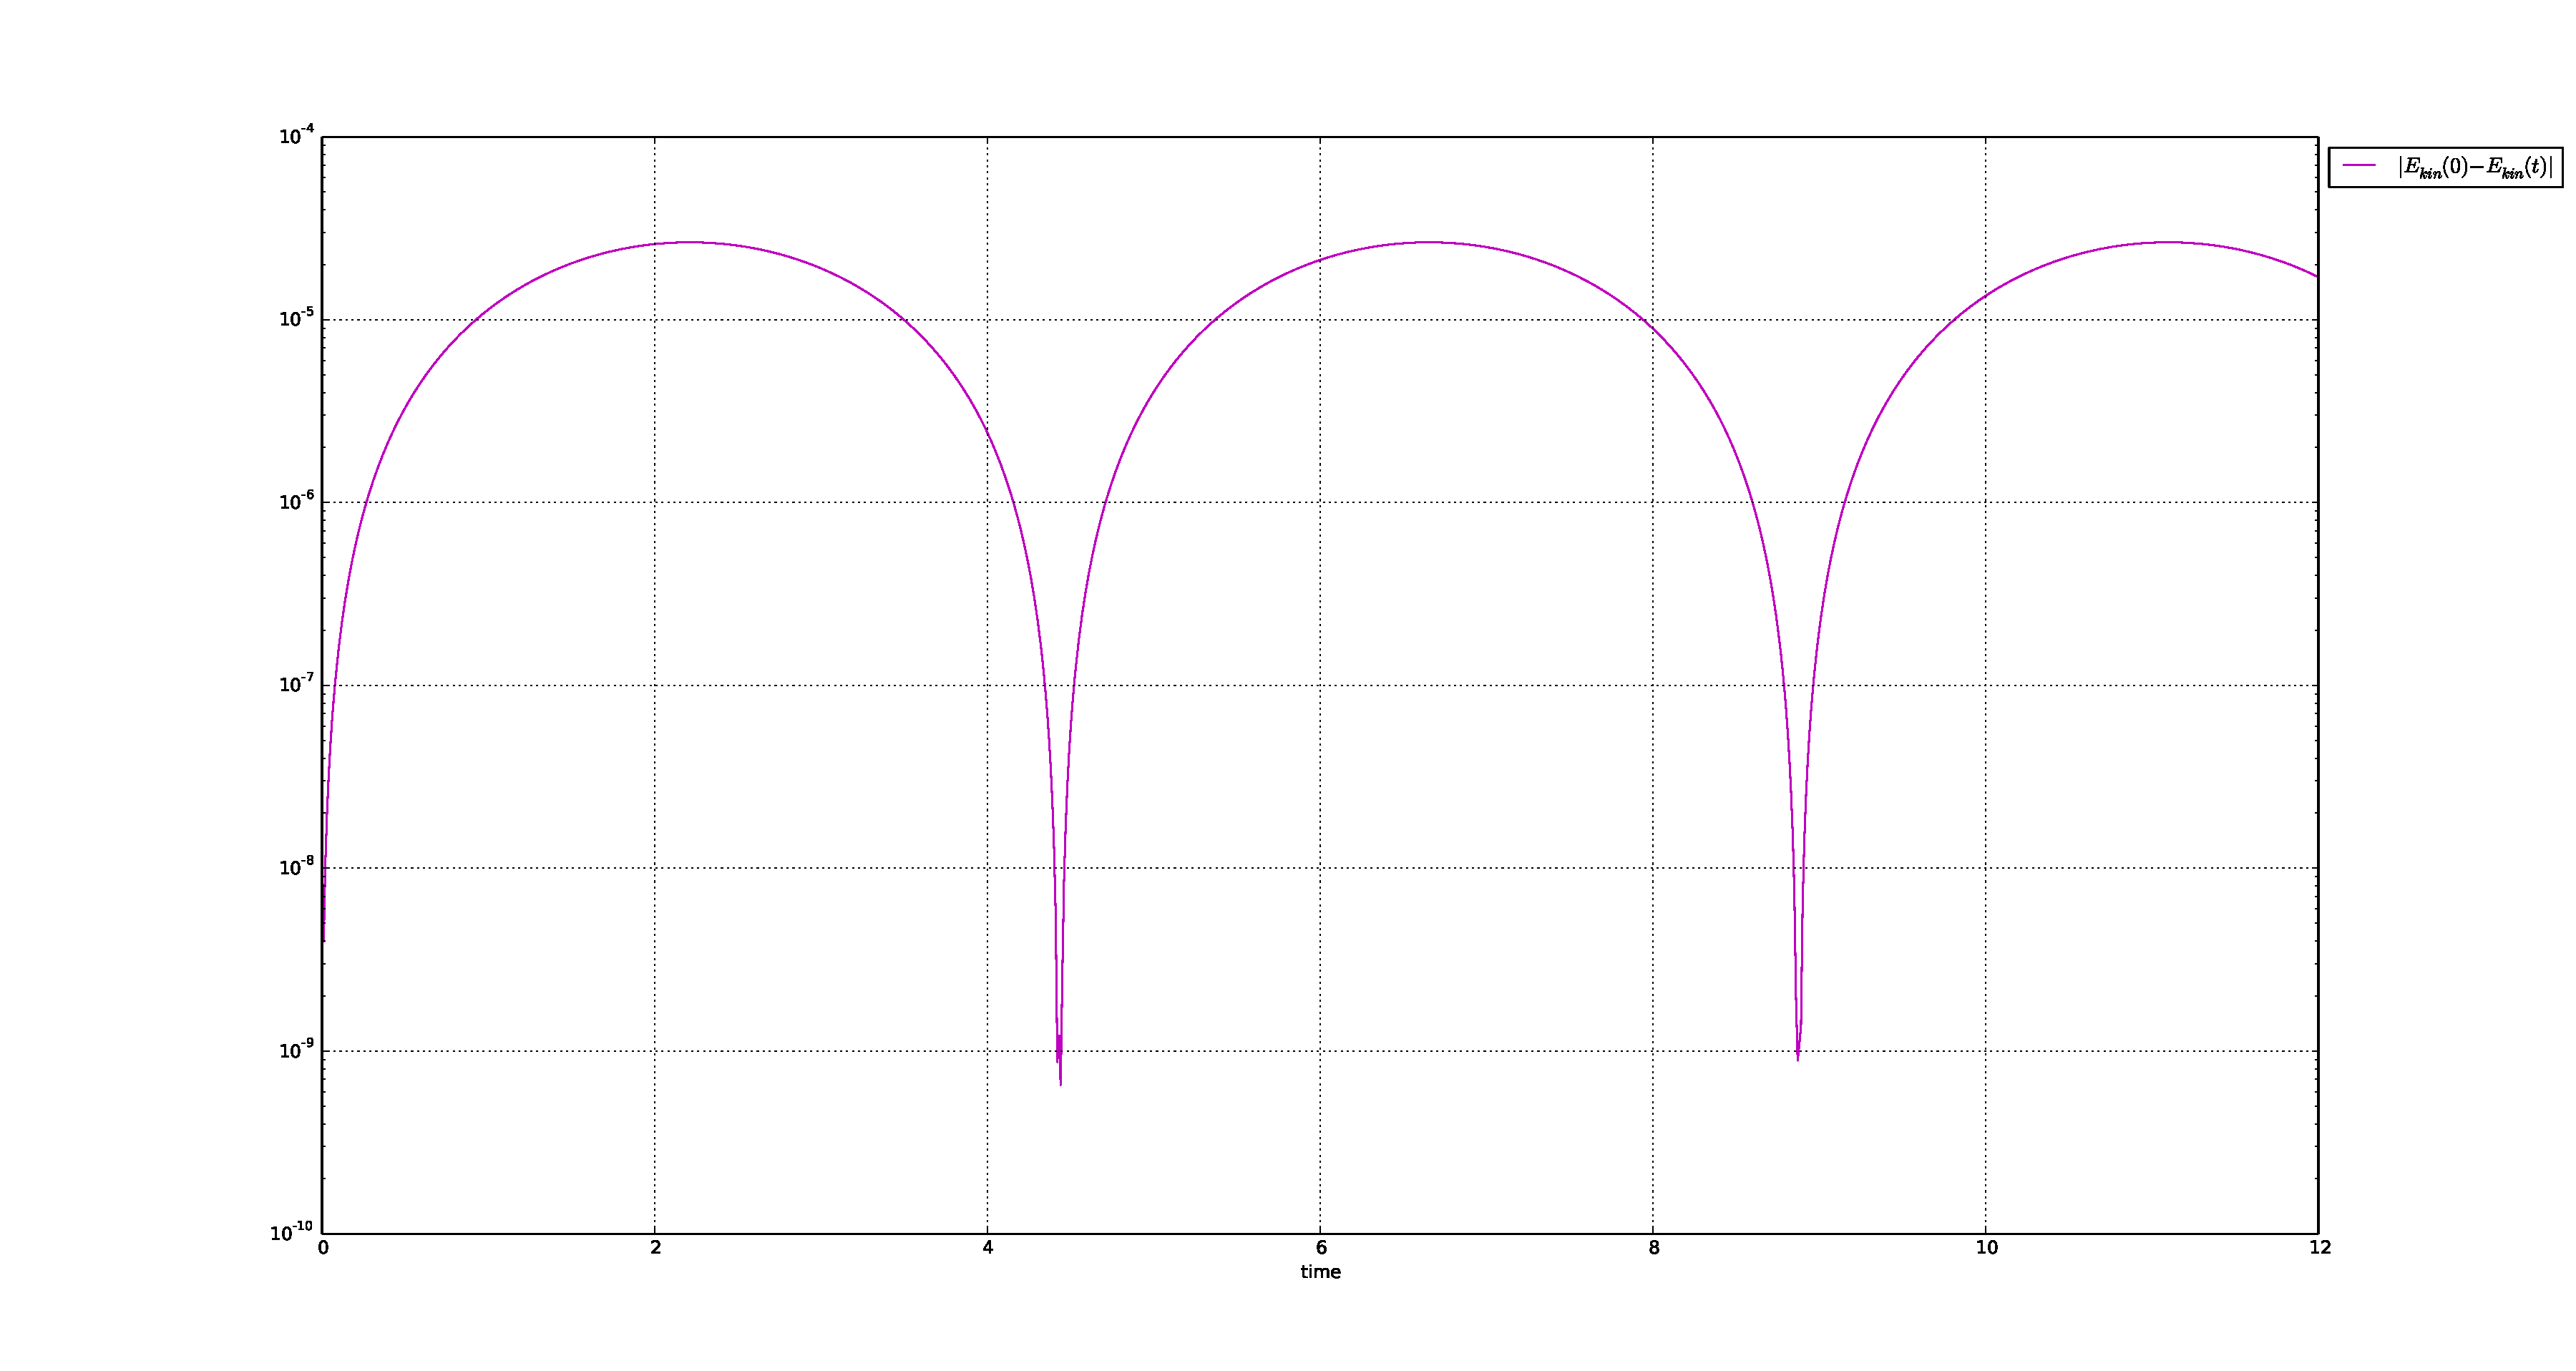
\includegraphics[width=\textwidth]{Figures/harmonic_drift.pdf}
\caption{The drift of the total energies in the harmonic simulation.}
\label{fig:harmonic_drift}
\end{figure}

\begin{figure}[!ht]
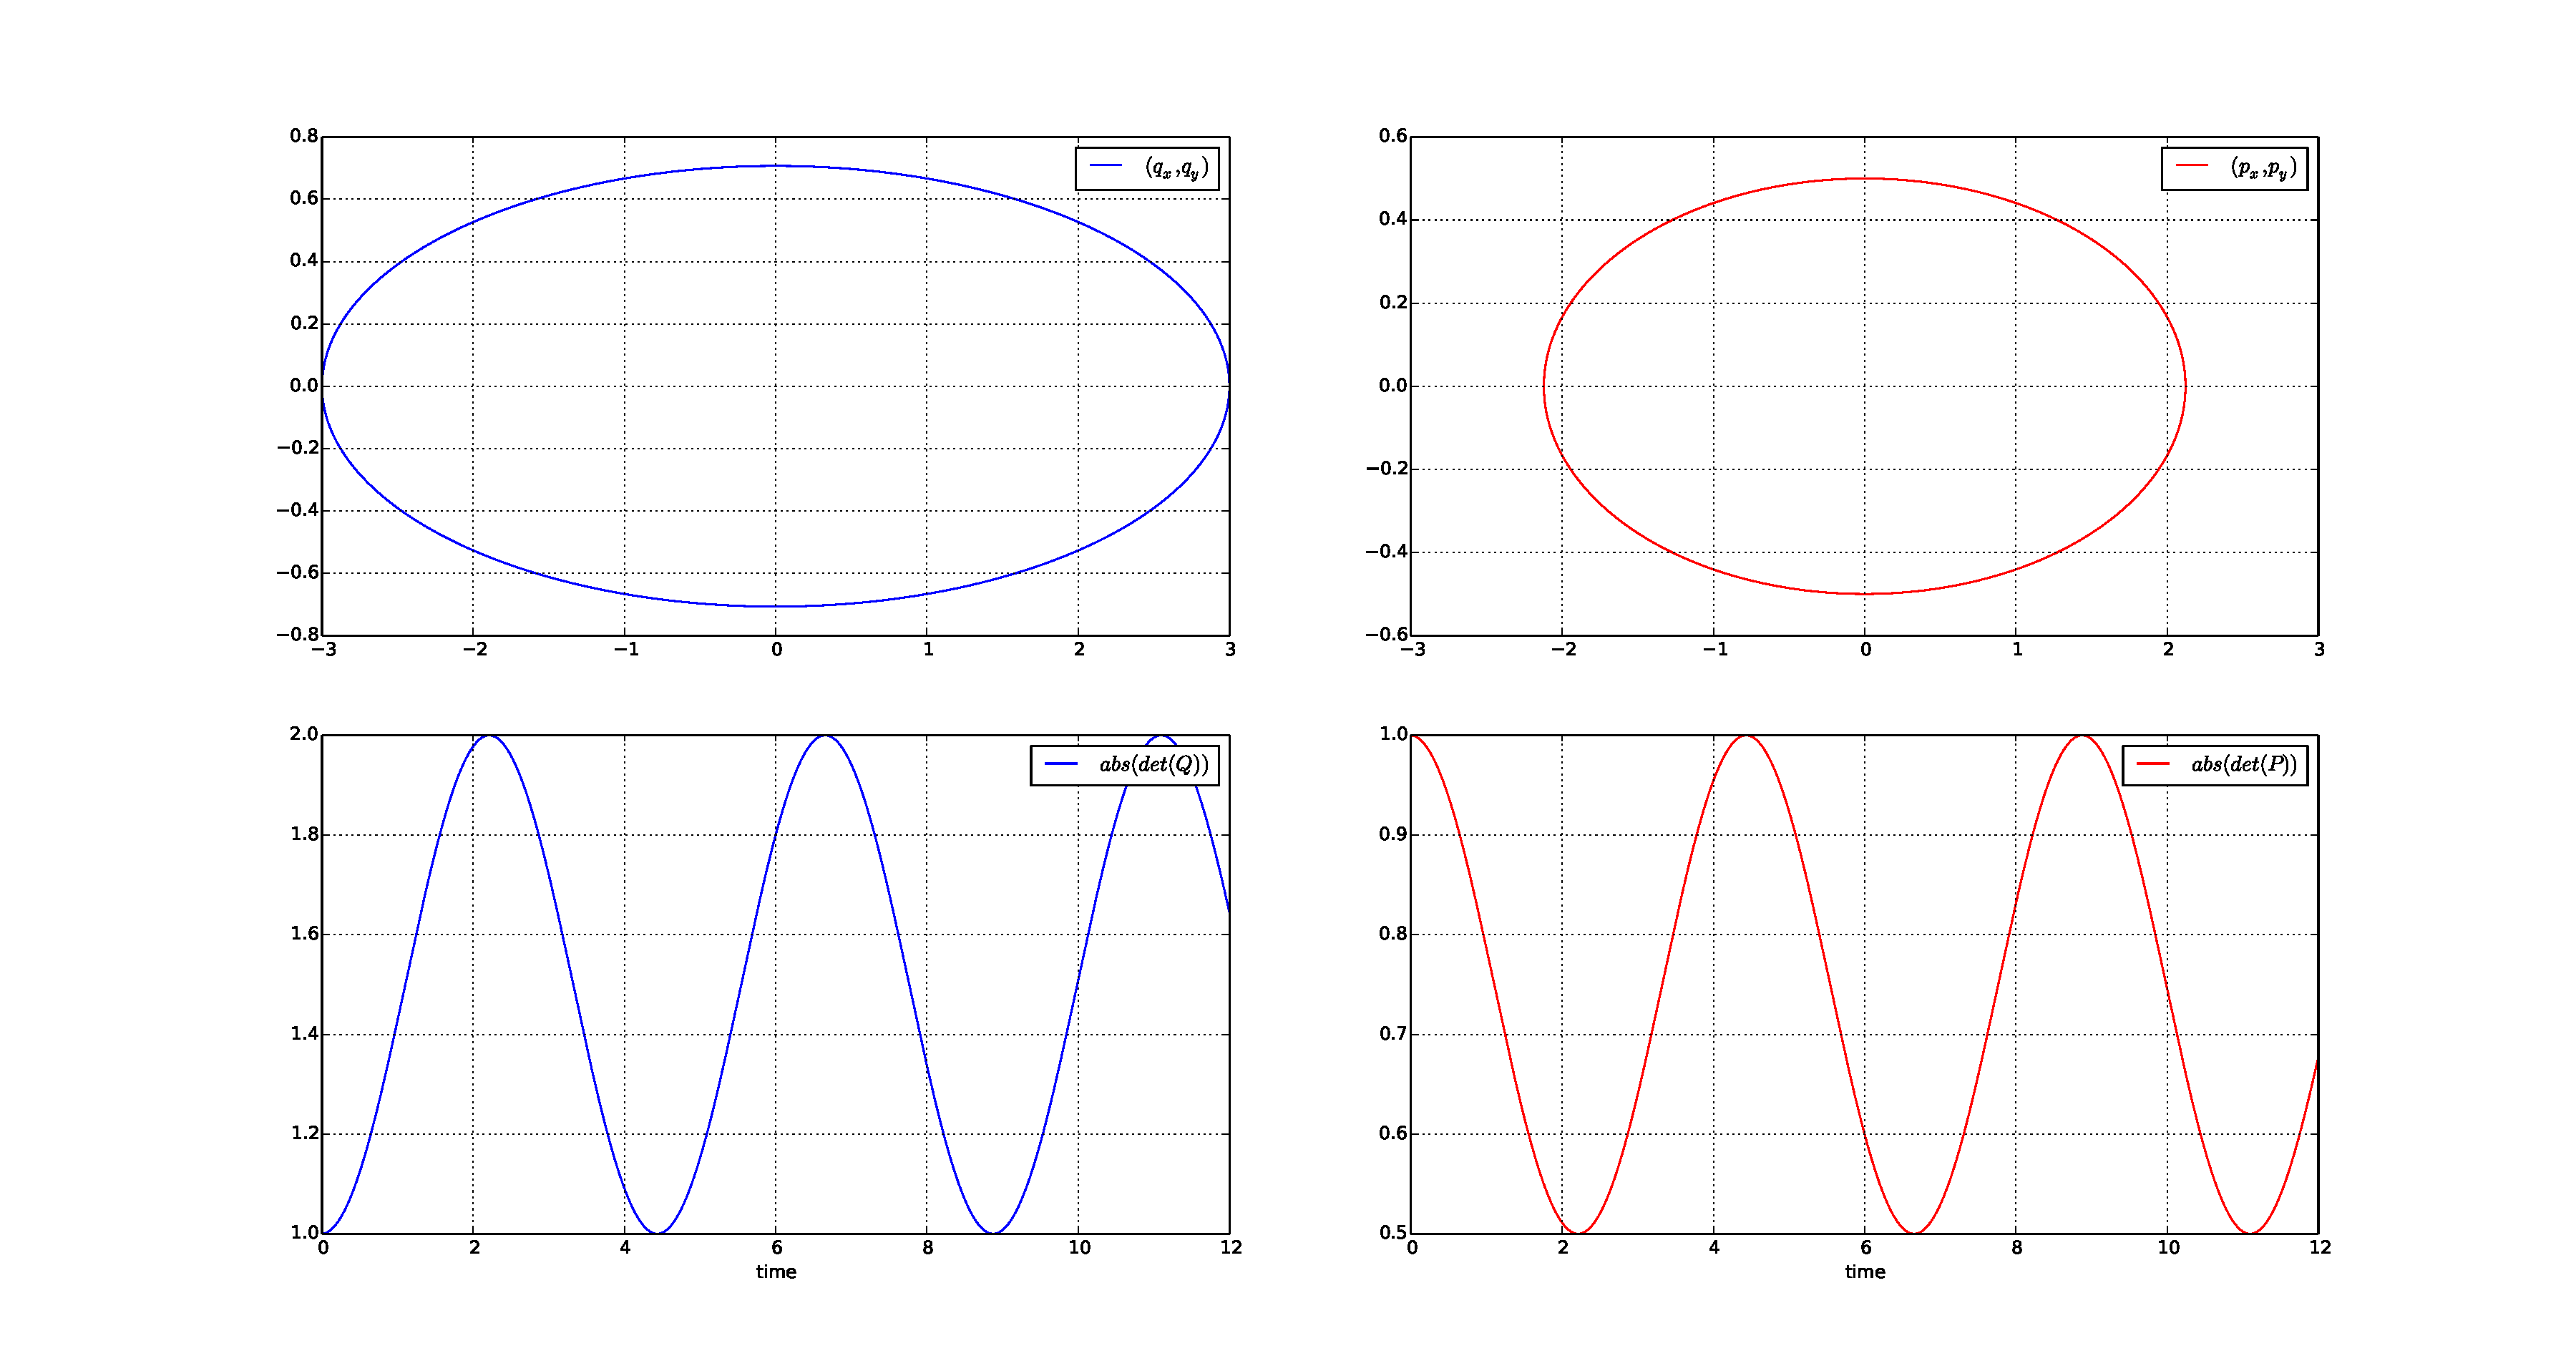
\includegraphics[width=\textwidth]{Figures/harmonic_params.pdf}
\caption{The position and momentum parameters of the harmonic simulation.}
\label{fig:harmonic_params}
\end{figure}
\begin{figure}[!ht]
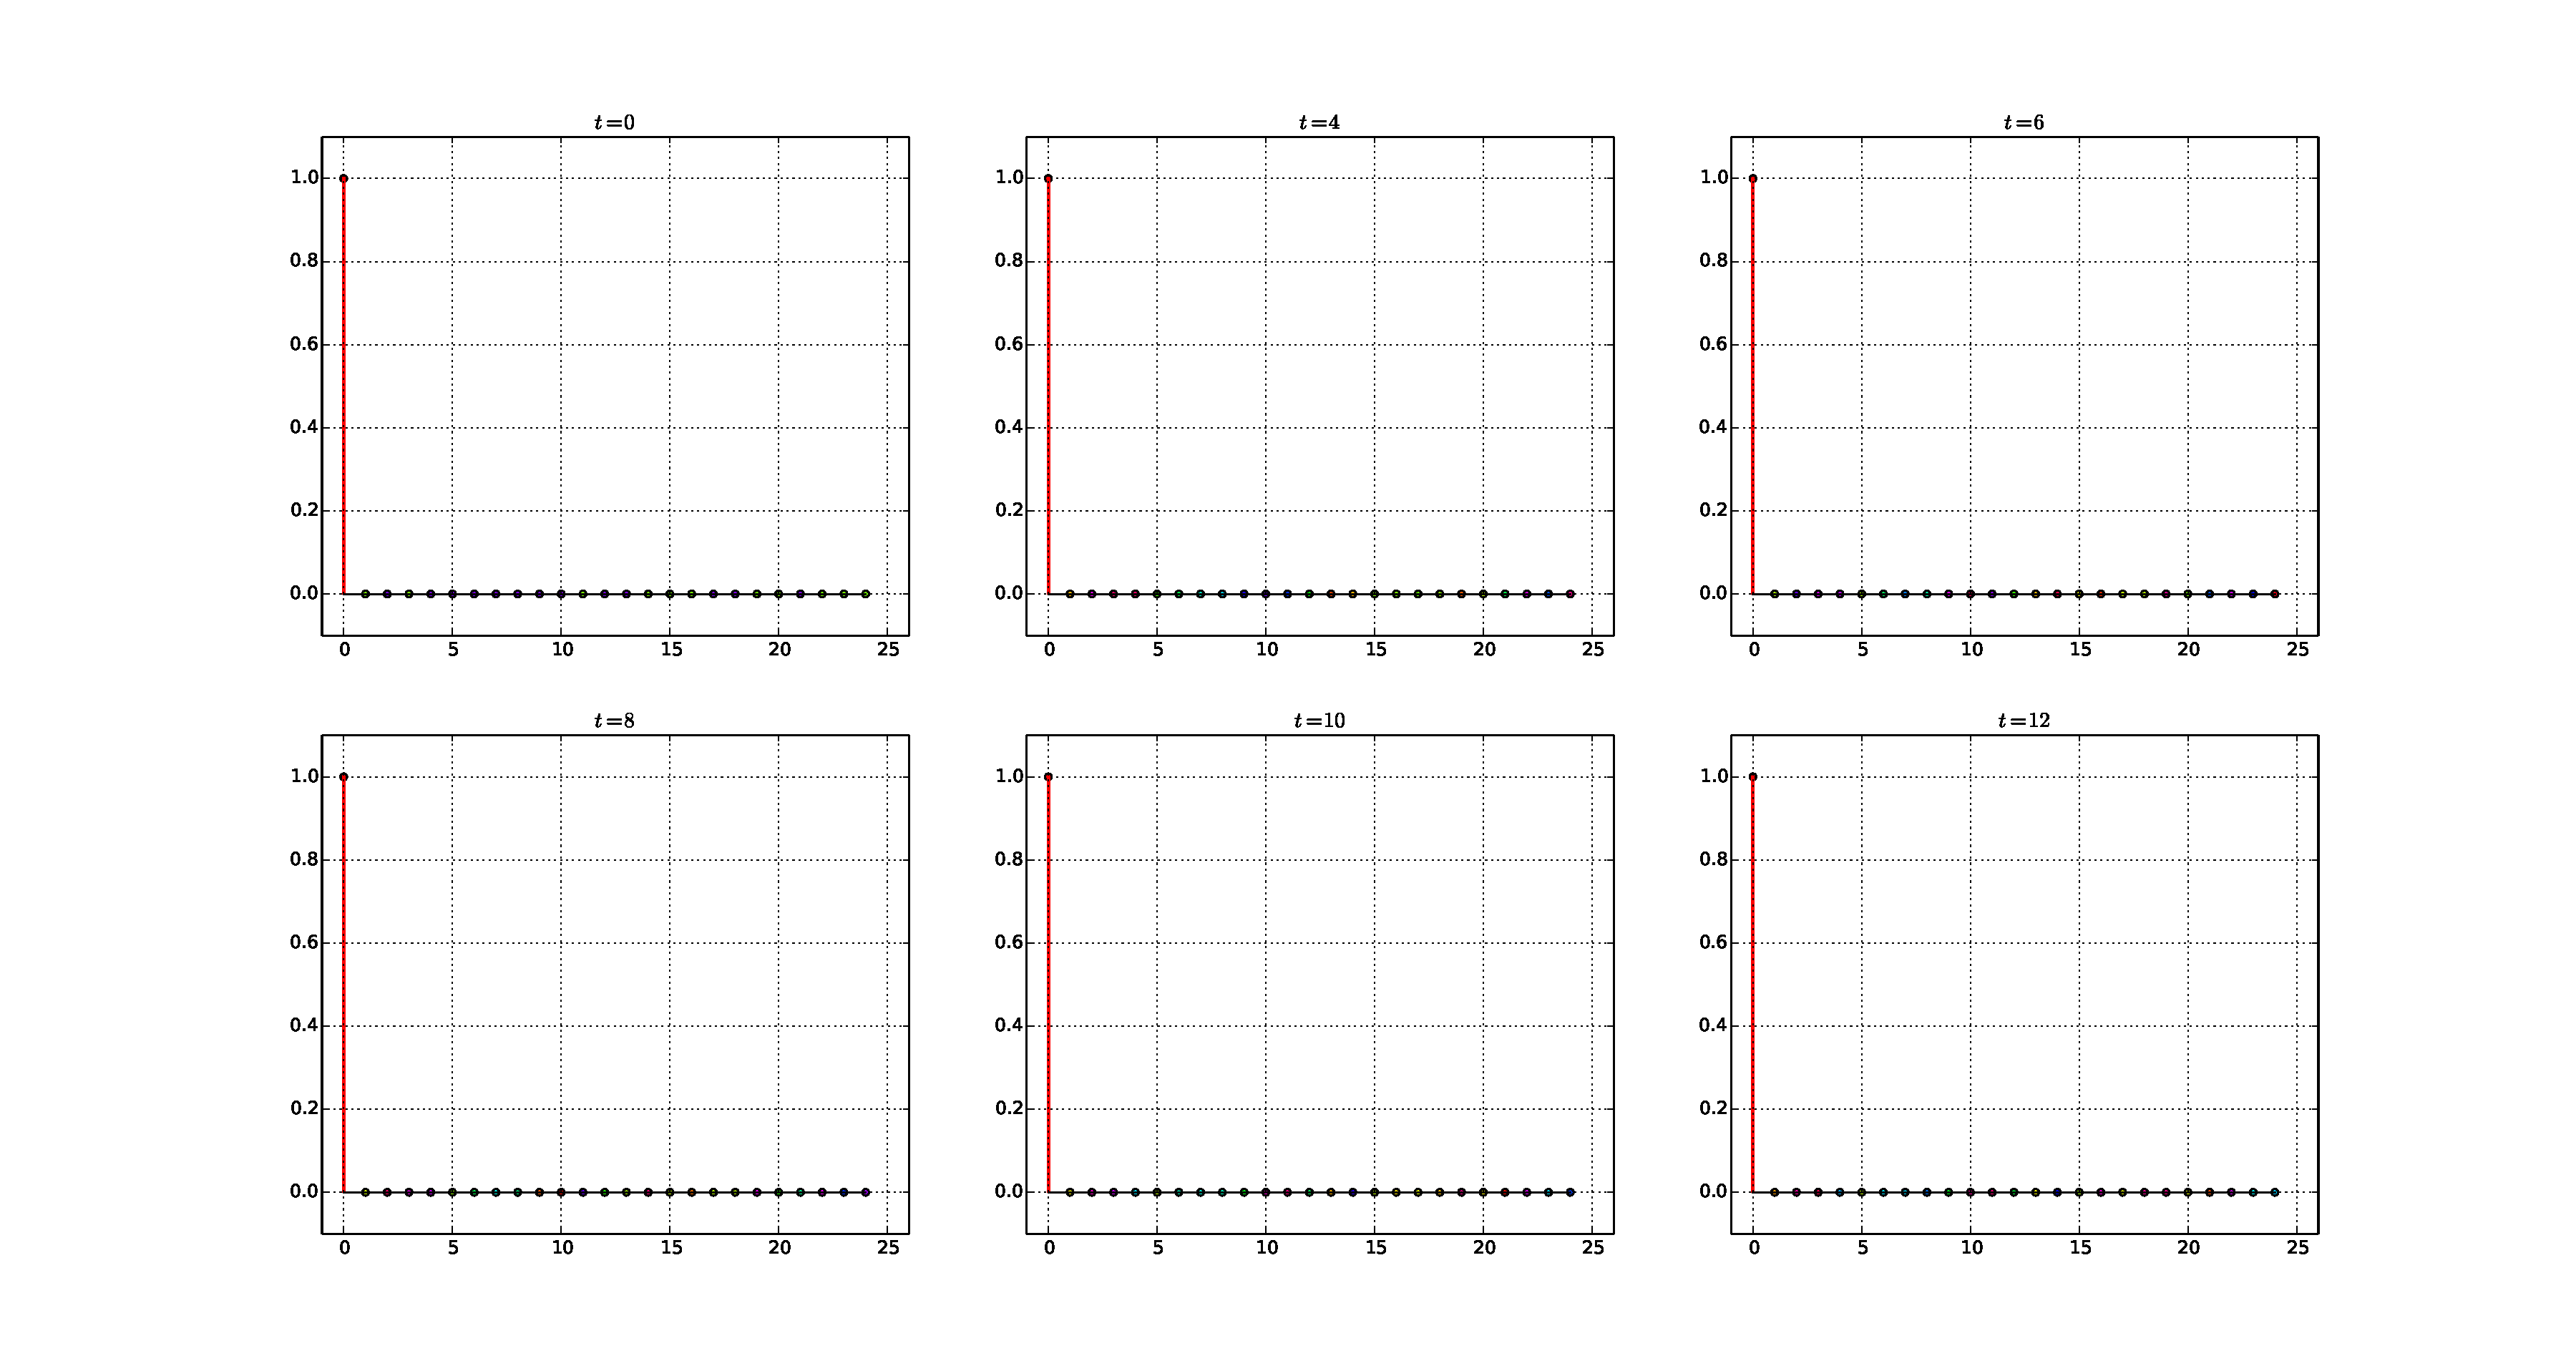
\includegraphics[width=\textwidth]{Figures/harmonic_coeffs.pdf}
\caption{The coefficients of the harmonic simulation.}
\label{fig:harmonic_coeffs}
\end{figure}

\FloatBarrier


\subsection{Anharmonic Oscillator}
This example considers the potential $V: \mathbb{R} \rightarrow \mathbb{R}$ where $V(x) = 1 + x^4$.

A Gaussian Hagedorn wavepacket with $128$ cubic shape basis functions with the following initial parameters:
\begin{center}
 \begin{tabular}{|c c c c c c|} 
 \hline
 q & p & Q & P & S & $\varepsilon$\\ [0.5ex] 
 \hline
 0 & 1 & 1 & i & 0 & 0.1\\ 
 \hline
\end{tabular}
\end{center}
is propagated using the Hagedorn propagator with $dt = 0.01$ up to $T = 6$.

Figure \ref{fig:anharmonic_drift} shows quite neat conservation of energy until the second reflection at which point the simulation seems to break down. This observation as well as the other plots are consistent with the \texttt{WaveBlocksND} implementation of the same example which serves as an indicator that the implementation is also correct in the anharmonic part.

\begin{figure}
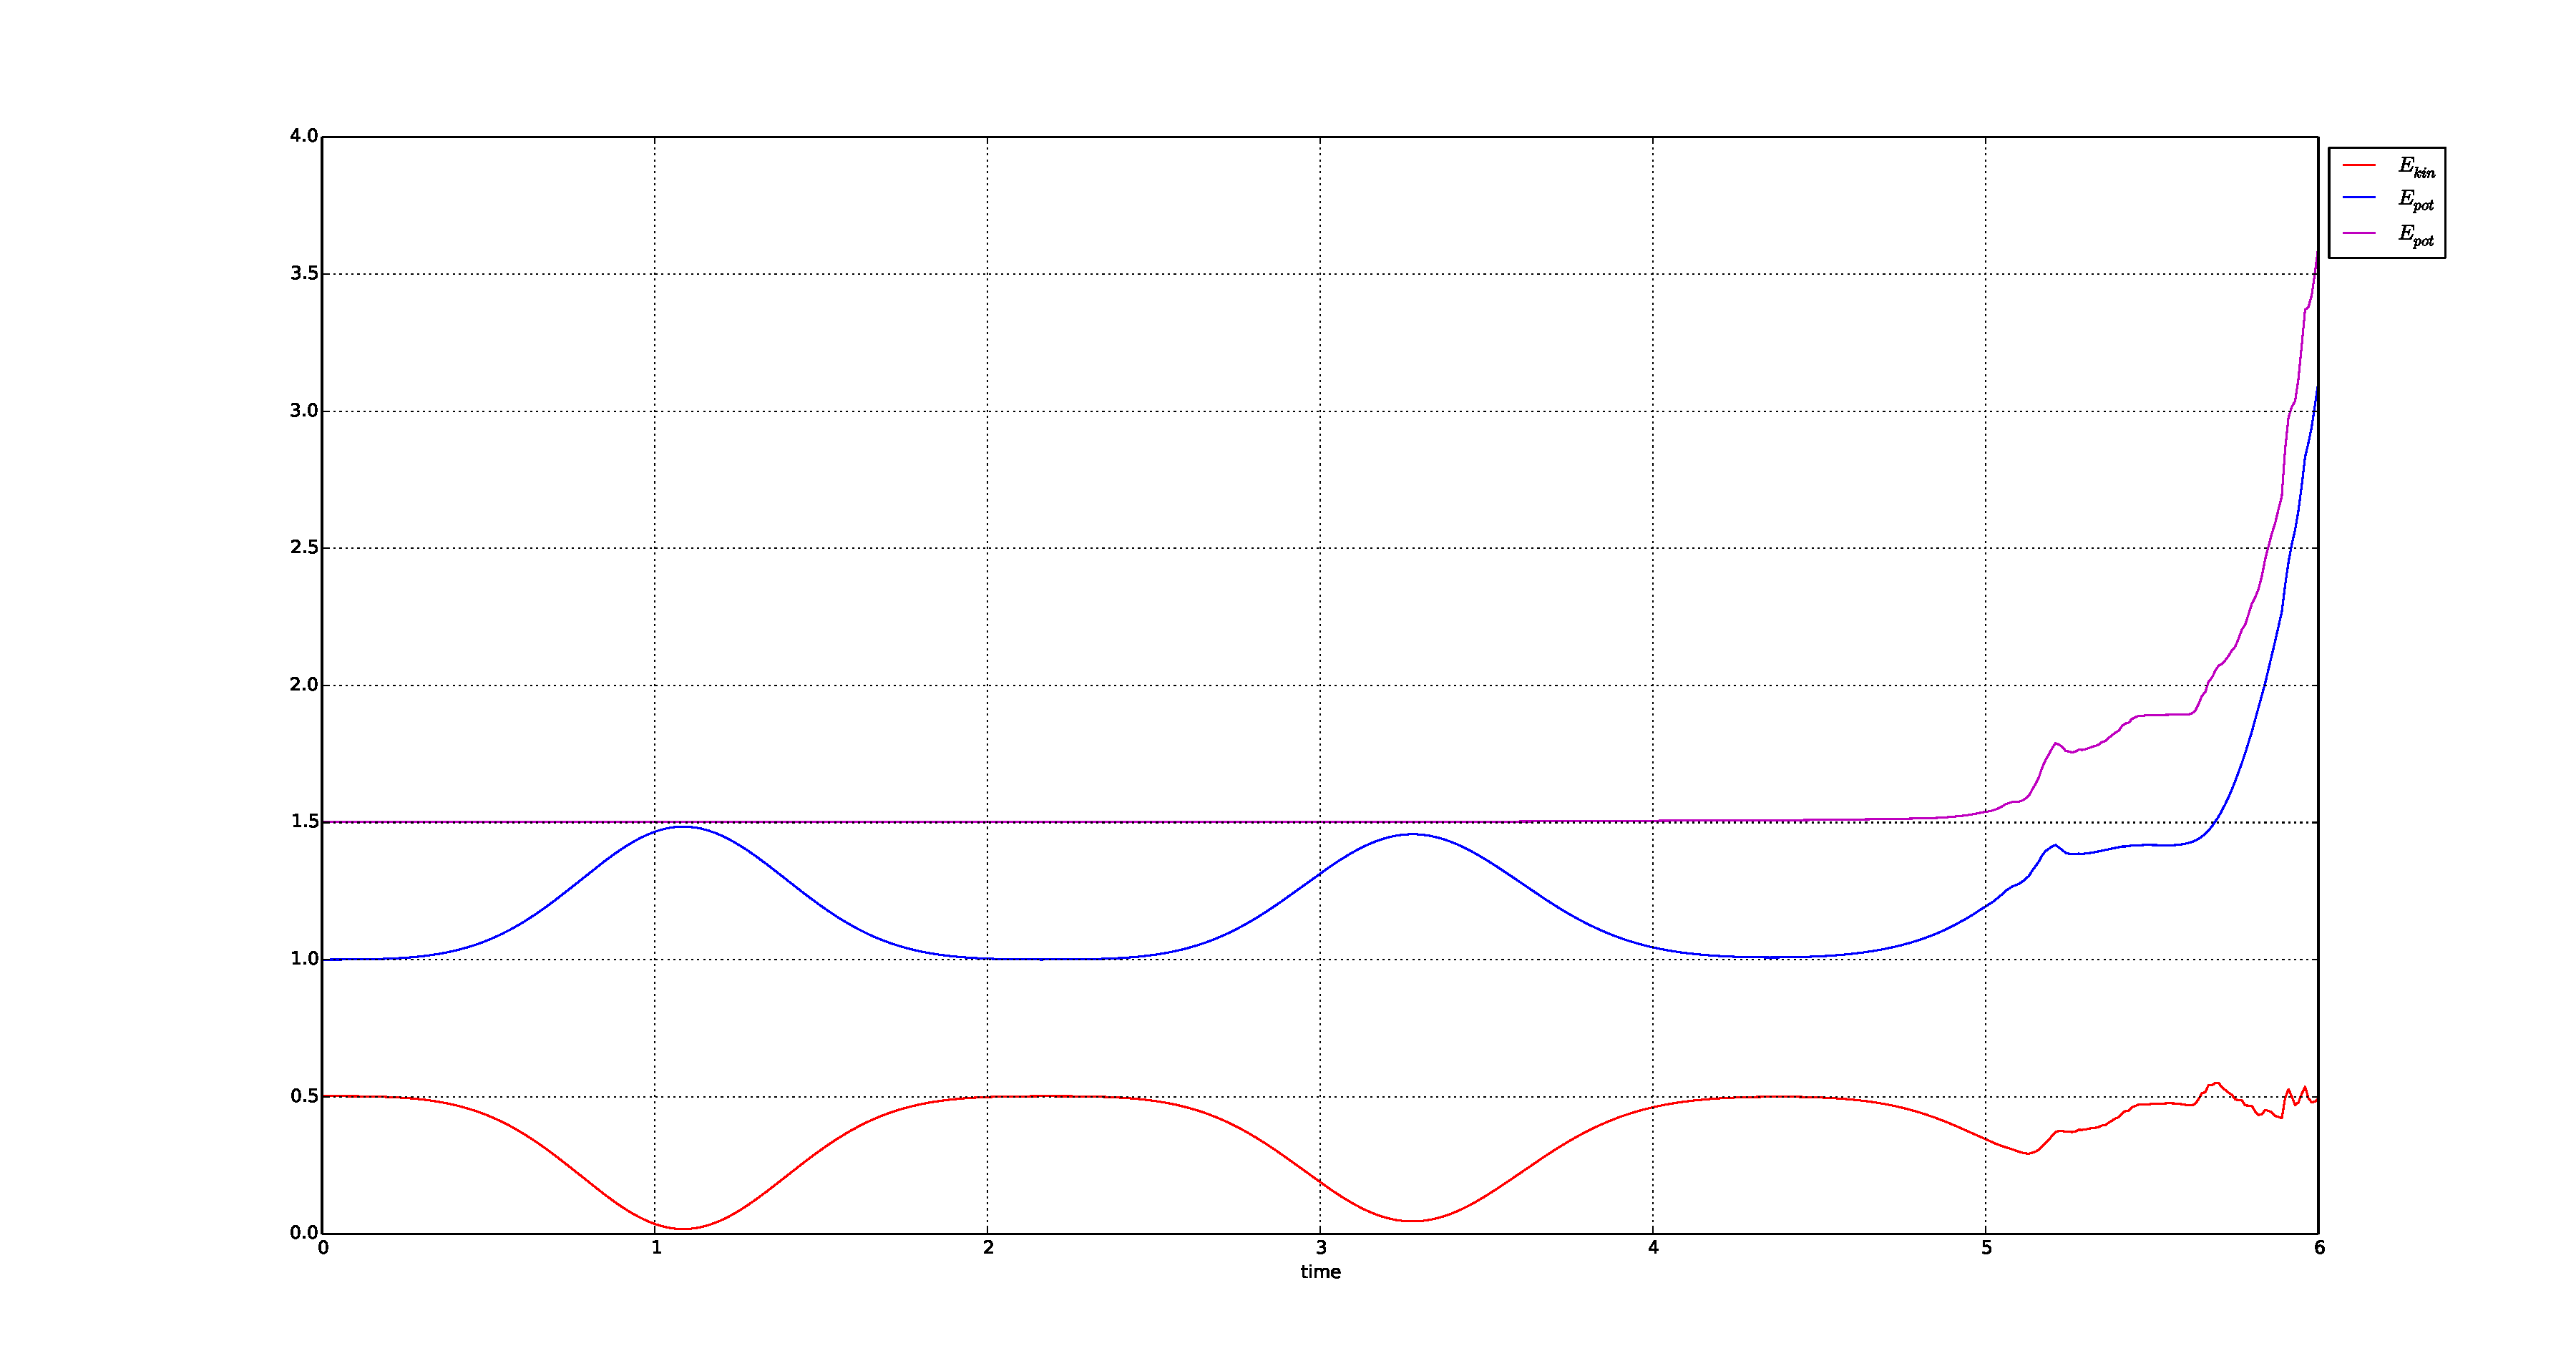
\includegraphics[width=\textwidth]{Figures/anharm_energy.pdf}
\caption{The energies of the anharmonic simulation.}
\label{fig:anharmonic_energy}
\end{figure}

\begin{figure}
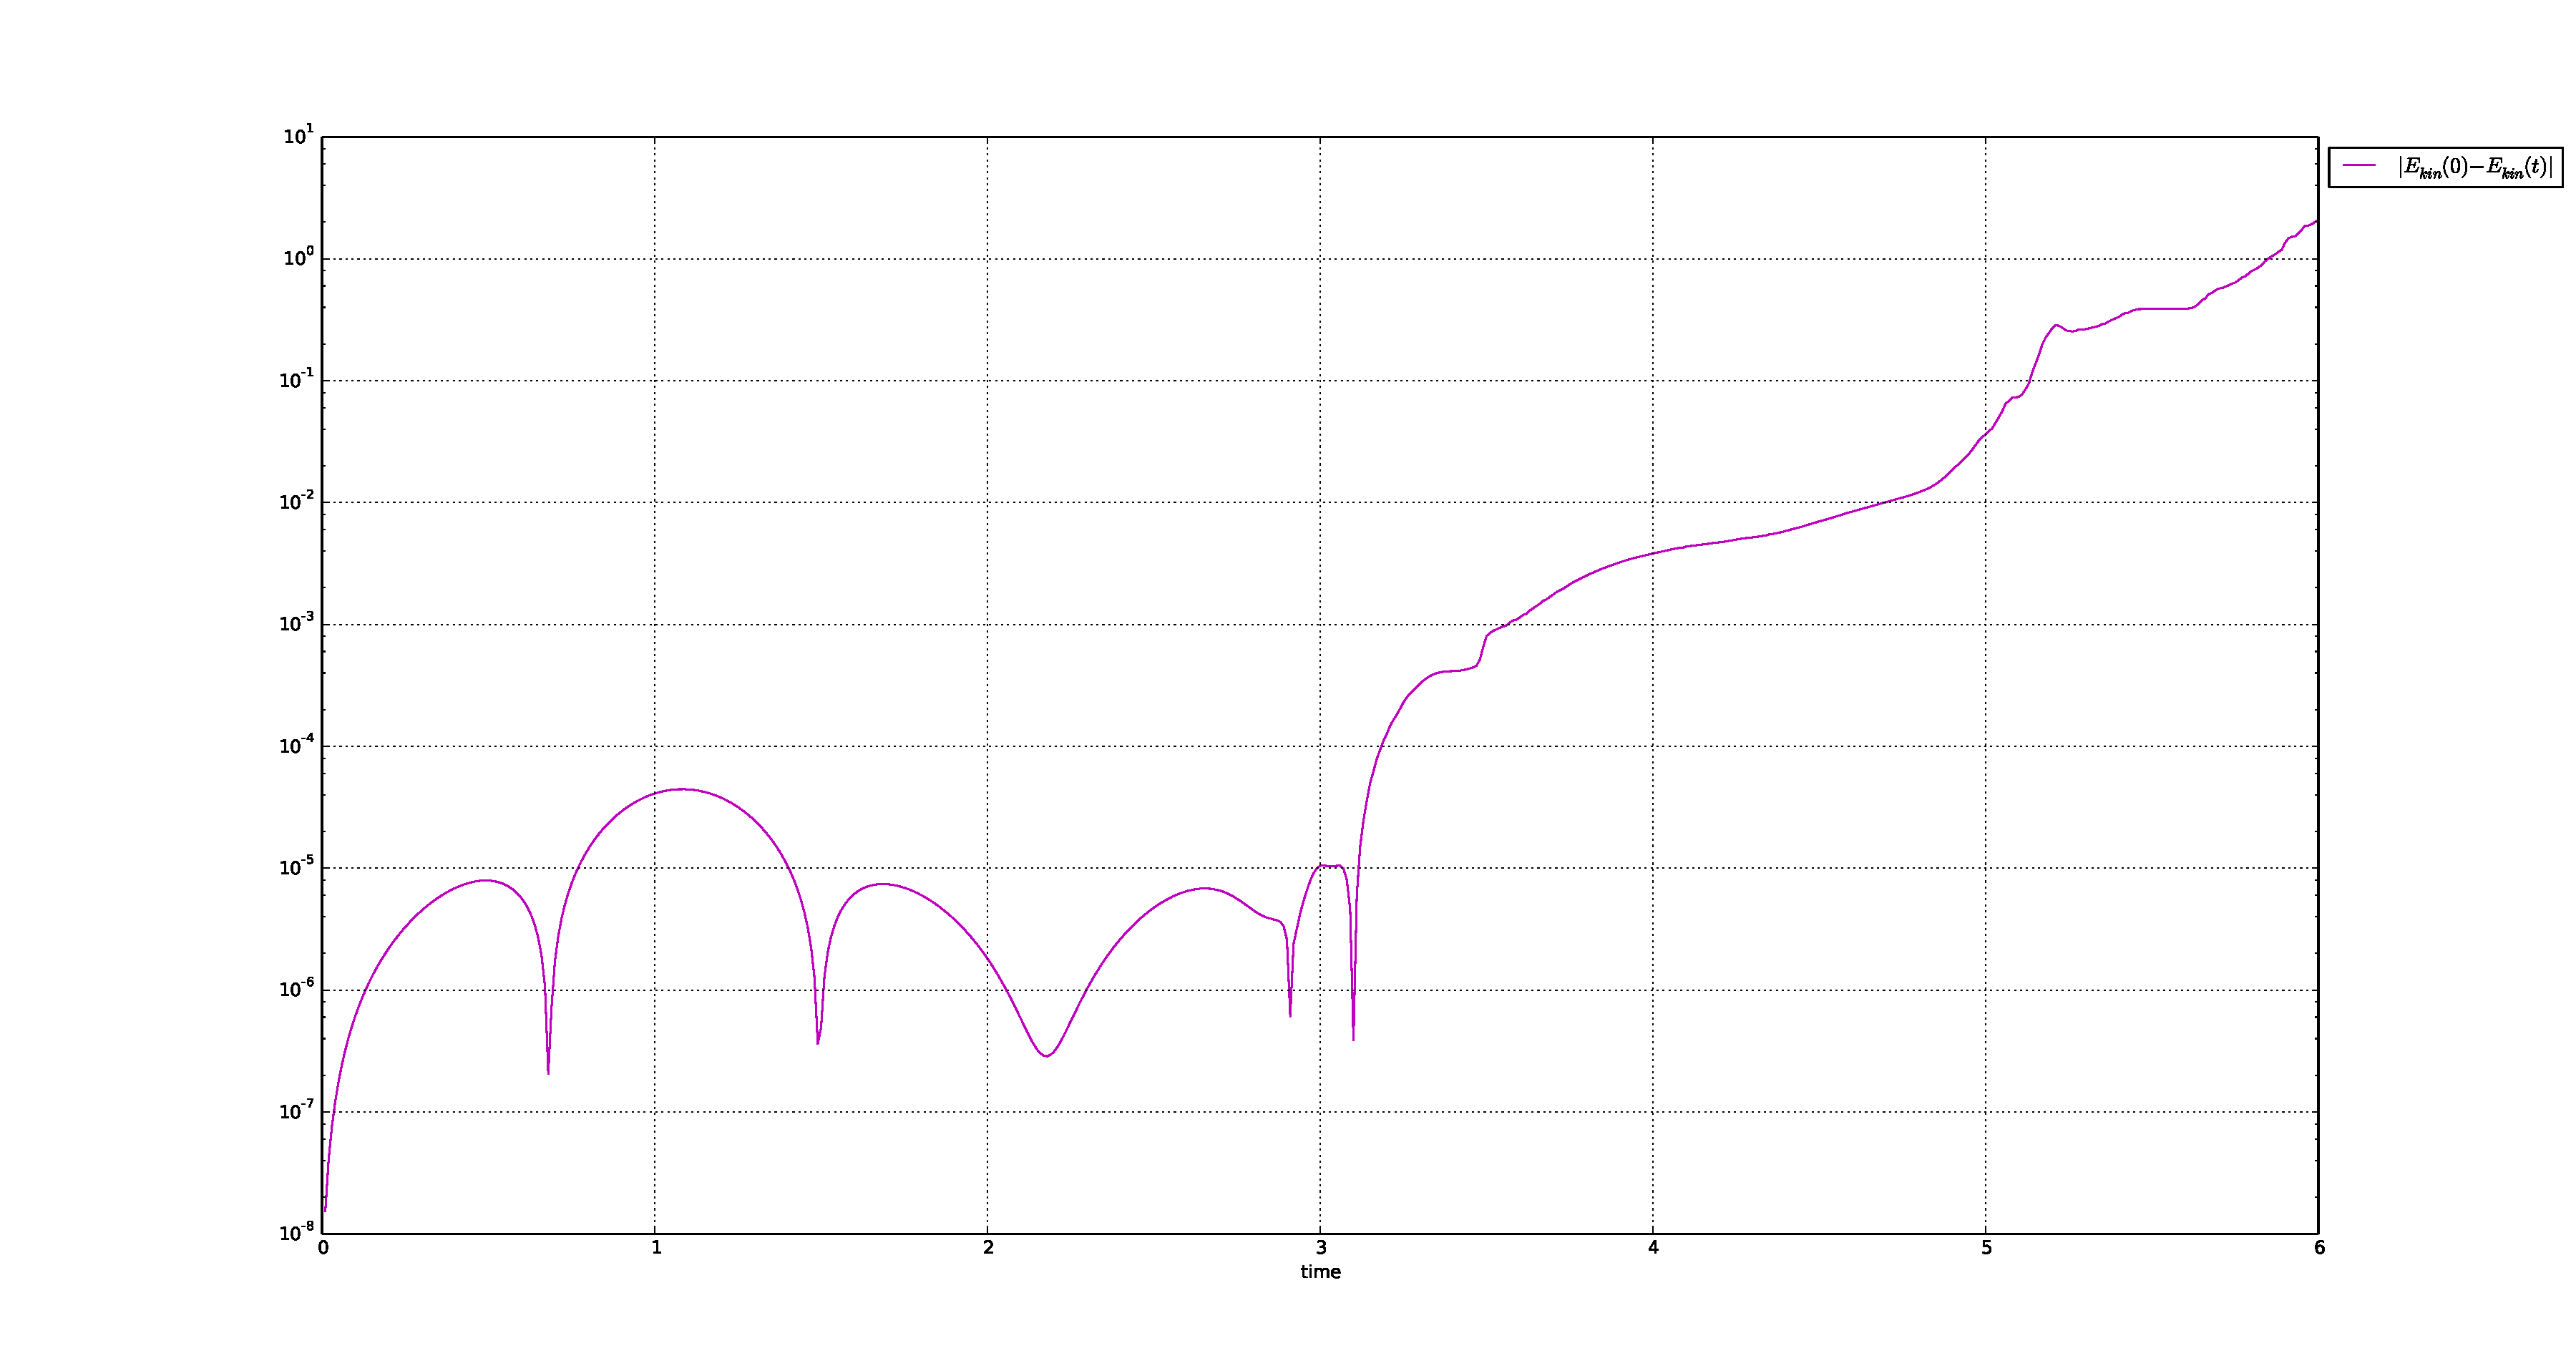
\includegraphics[width=\textwidth]{Figures/anharmonic_drift.pdf}
\caption{The drift of the total energies in the anharmonic simulation.}
\label{fig:anharmonic_drift}
\end{figure}

\begin{figure}
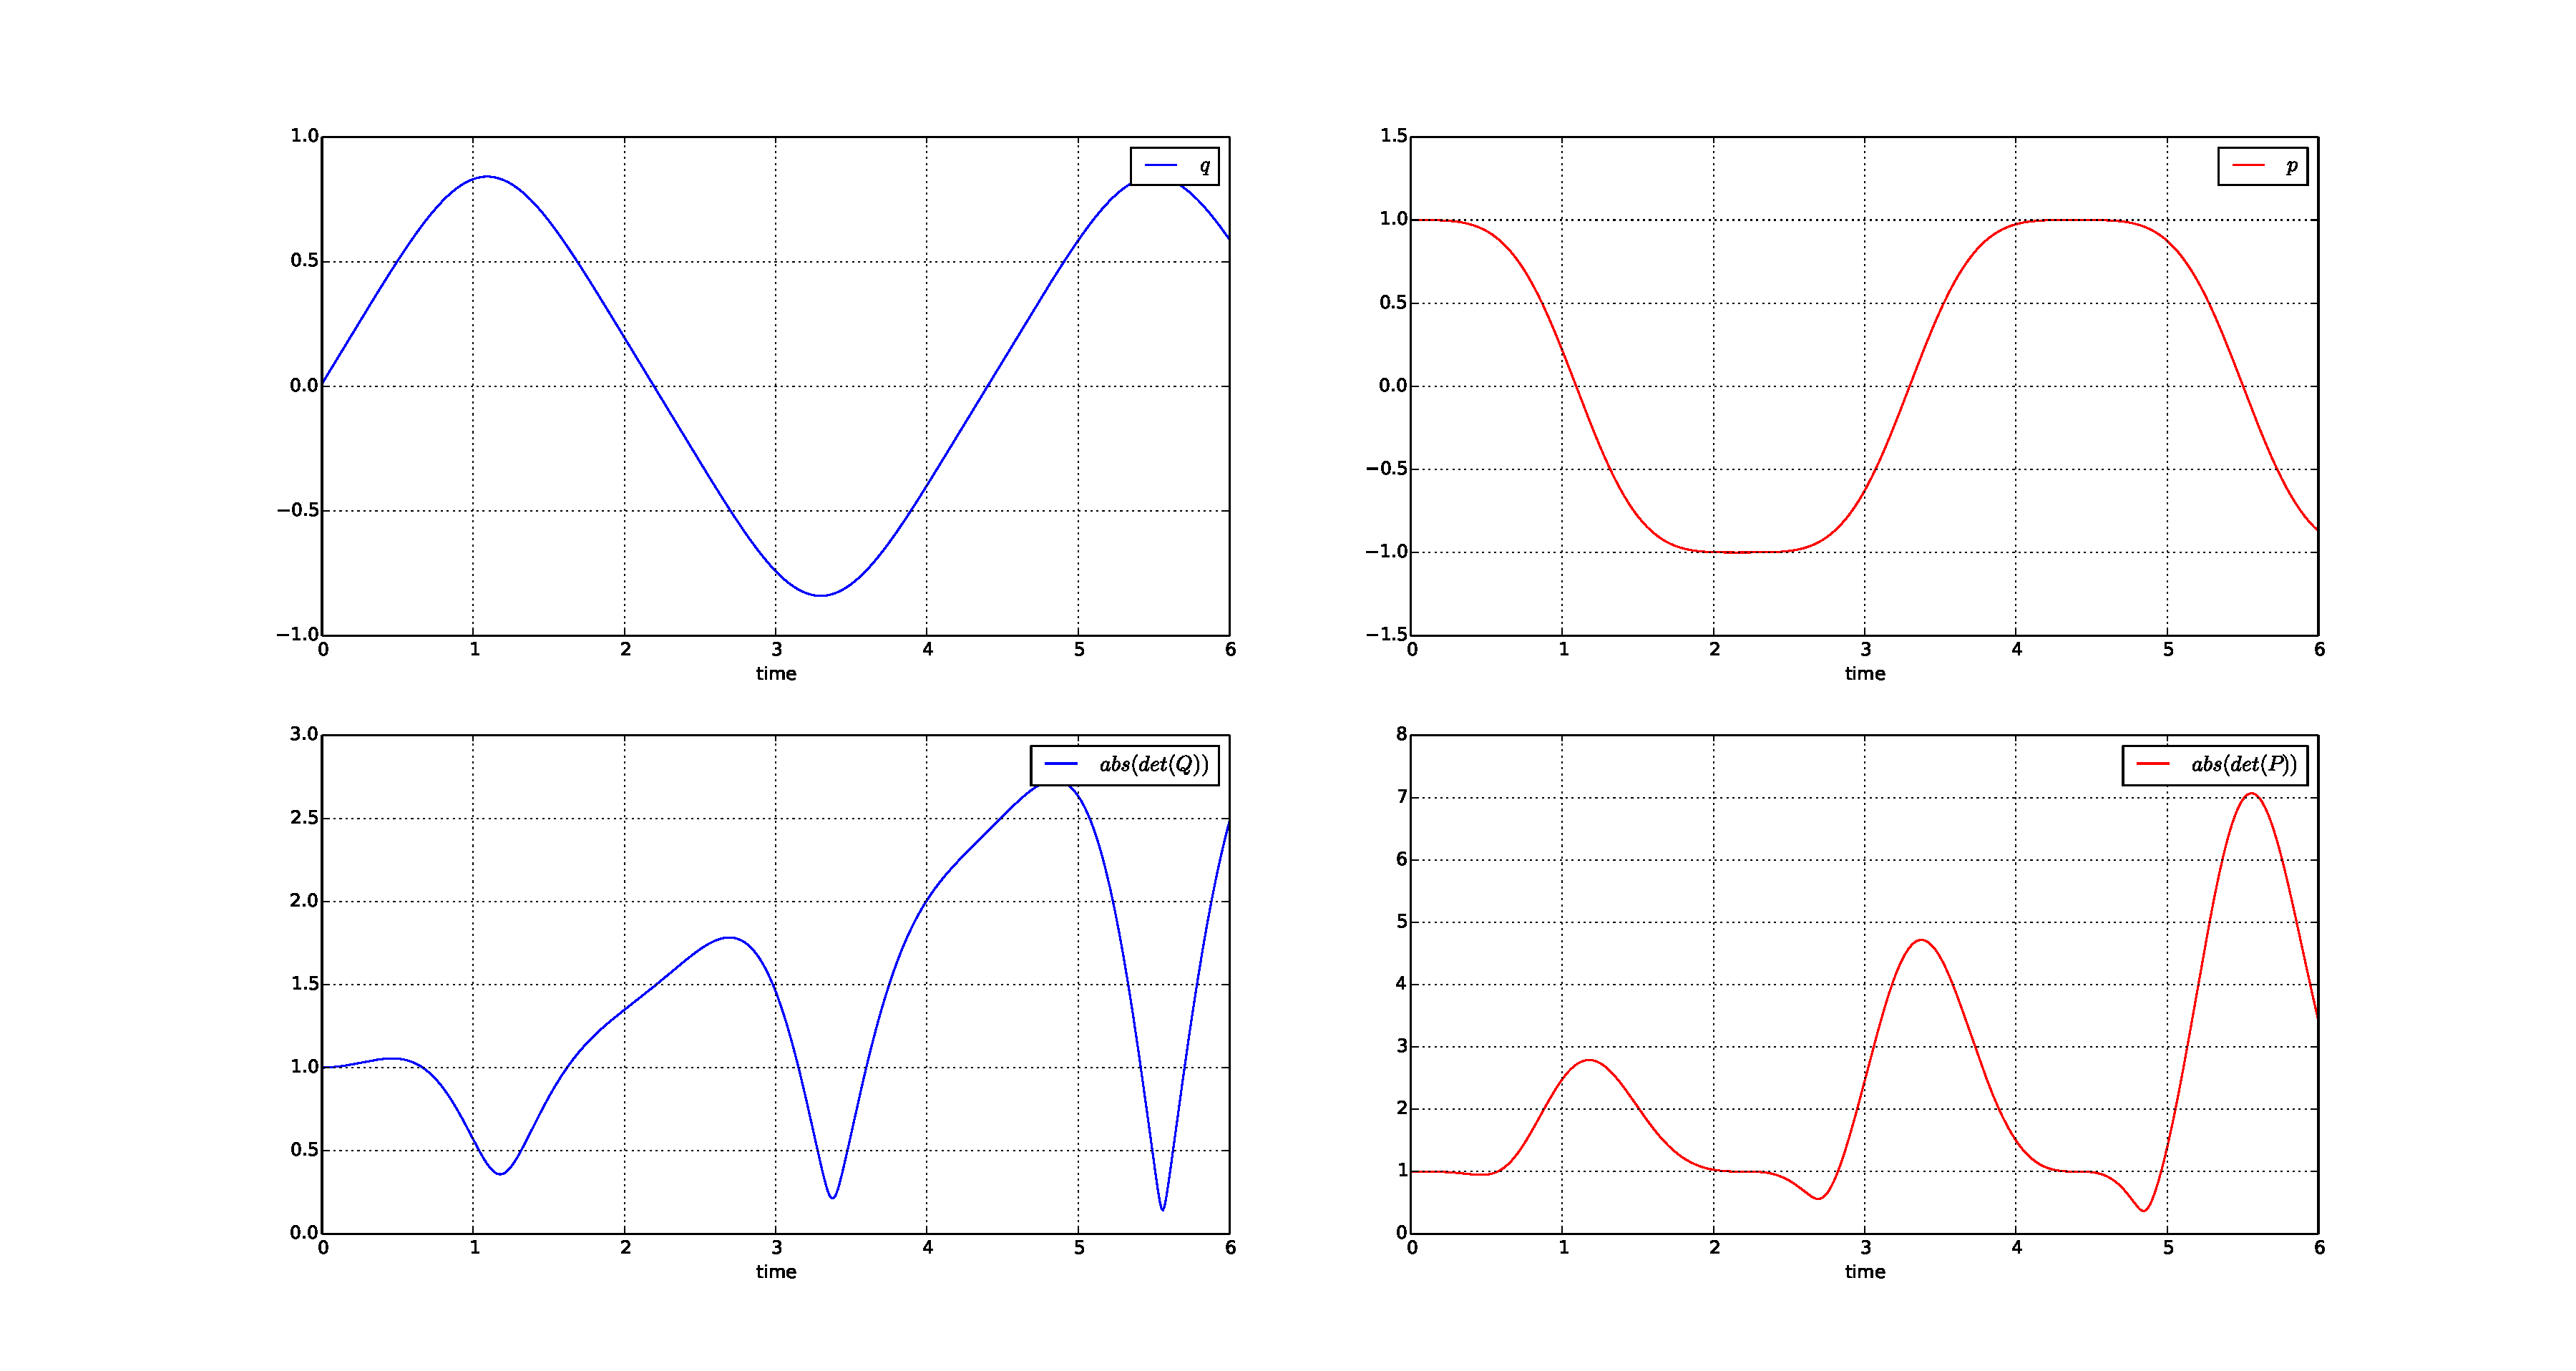
\includegraphics[width=\textwidth]{Figures/anharm_params.pdf}
\caption{The position and momentum parameters of the harmonic simulation.}
\end{figure}
\begin{figure}
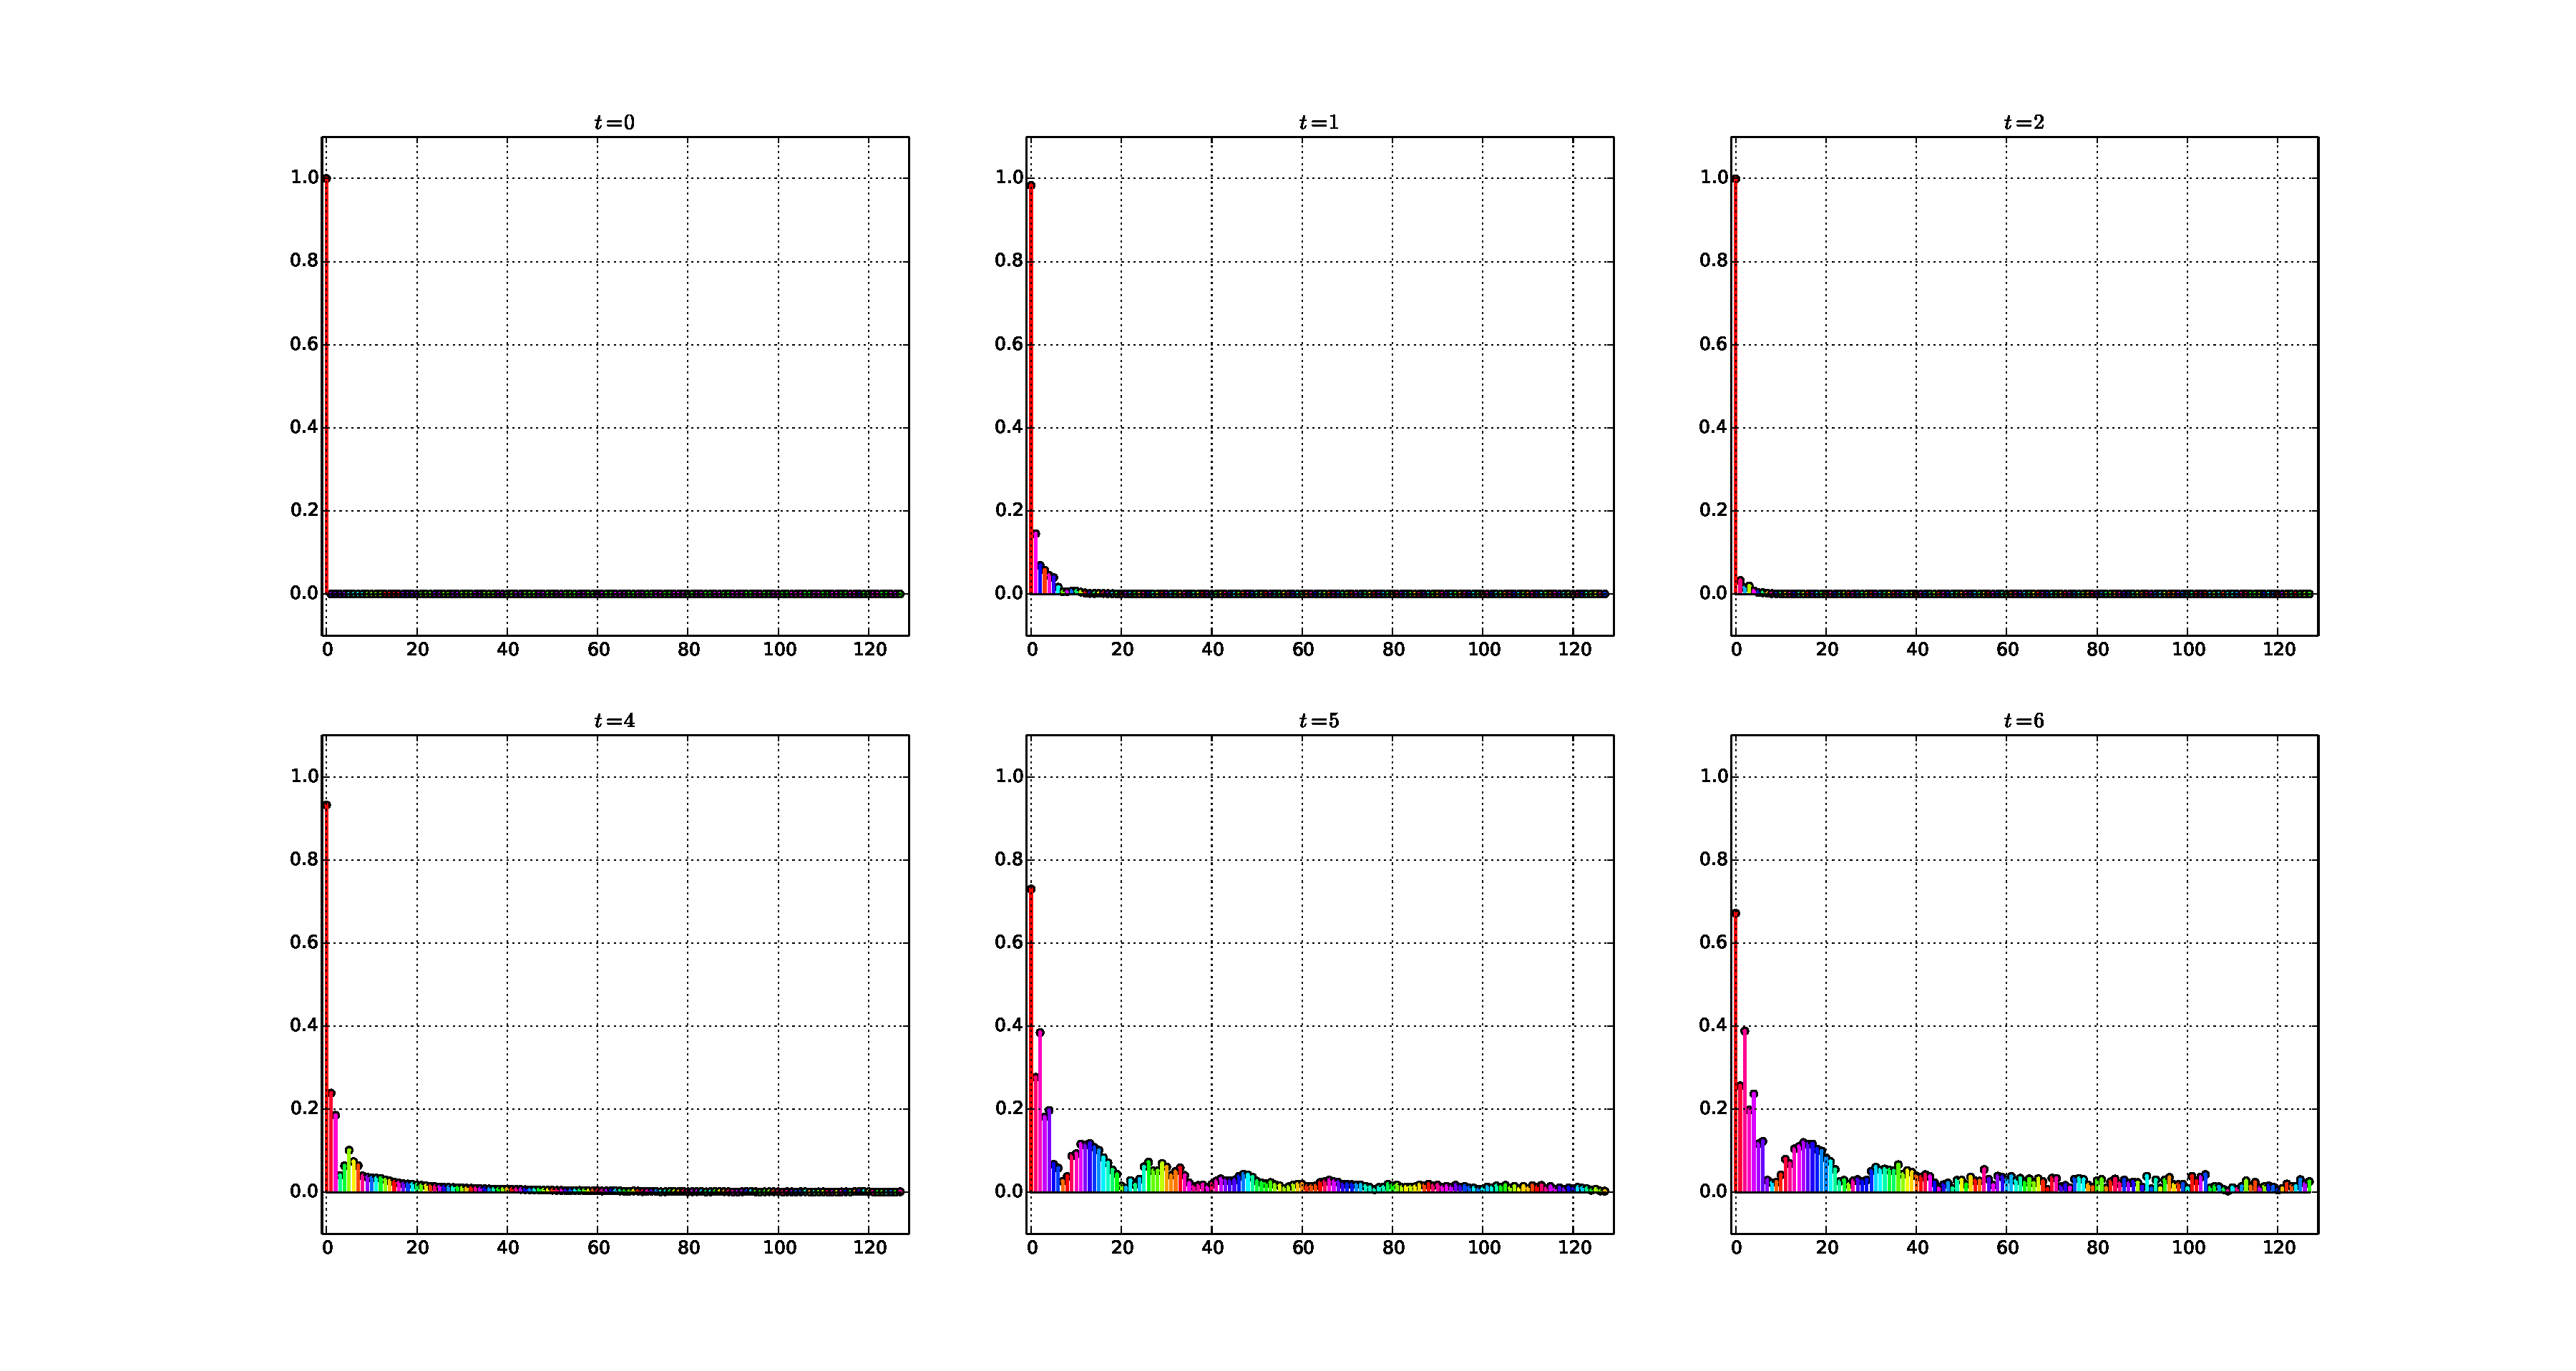
\includegraphics[width=\textwidth]{Figures/anharm_coeffs.pdf}
\caption{The coefficients of the harmonic simulation.}
\end{figure}
\FloatBarrier

\subsection{Conclusion}
Both simulations were consistent with the \texttt{WaveBlocksND} implementation which gives confidence that the implementation is correct for $N=1$.

\section{1D Tunneling}
I attempt to recompute the simulation in \cite{GHJ_tunneling_spawning} as an application of the \texttt{C++} framework.
\subsection{Setup}
Consider the scalar potential $V: \mathbb{R} \rightarrow \mathbb{R}$ with $V(x) = { \sigma \over \cosh(x/a)^2 }$, where $\sigma = 100 {\text{kJ} \over \text{mol}} = 0.038088 \text{ Eh}$ and $a = 0.5\text{ \r{A}} = 0.944858 \text{ alu}$ (as in Figure \ref{fig:tunneling_pot}). 
\begin{figure}
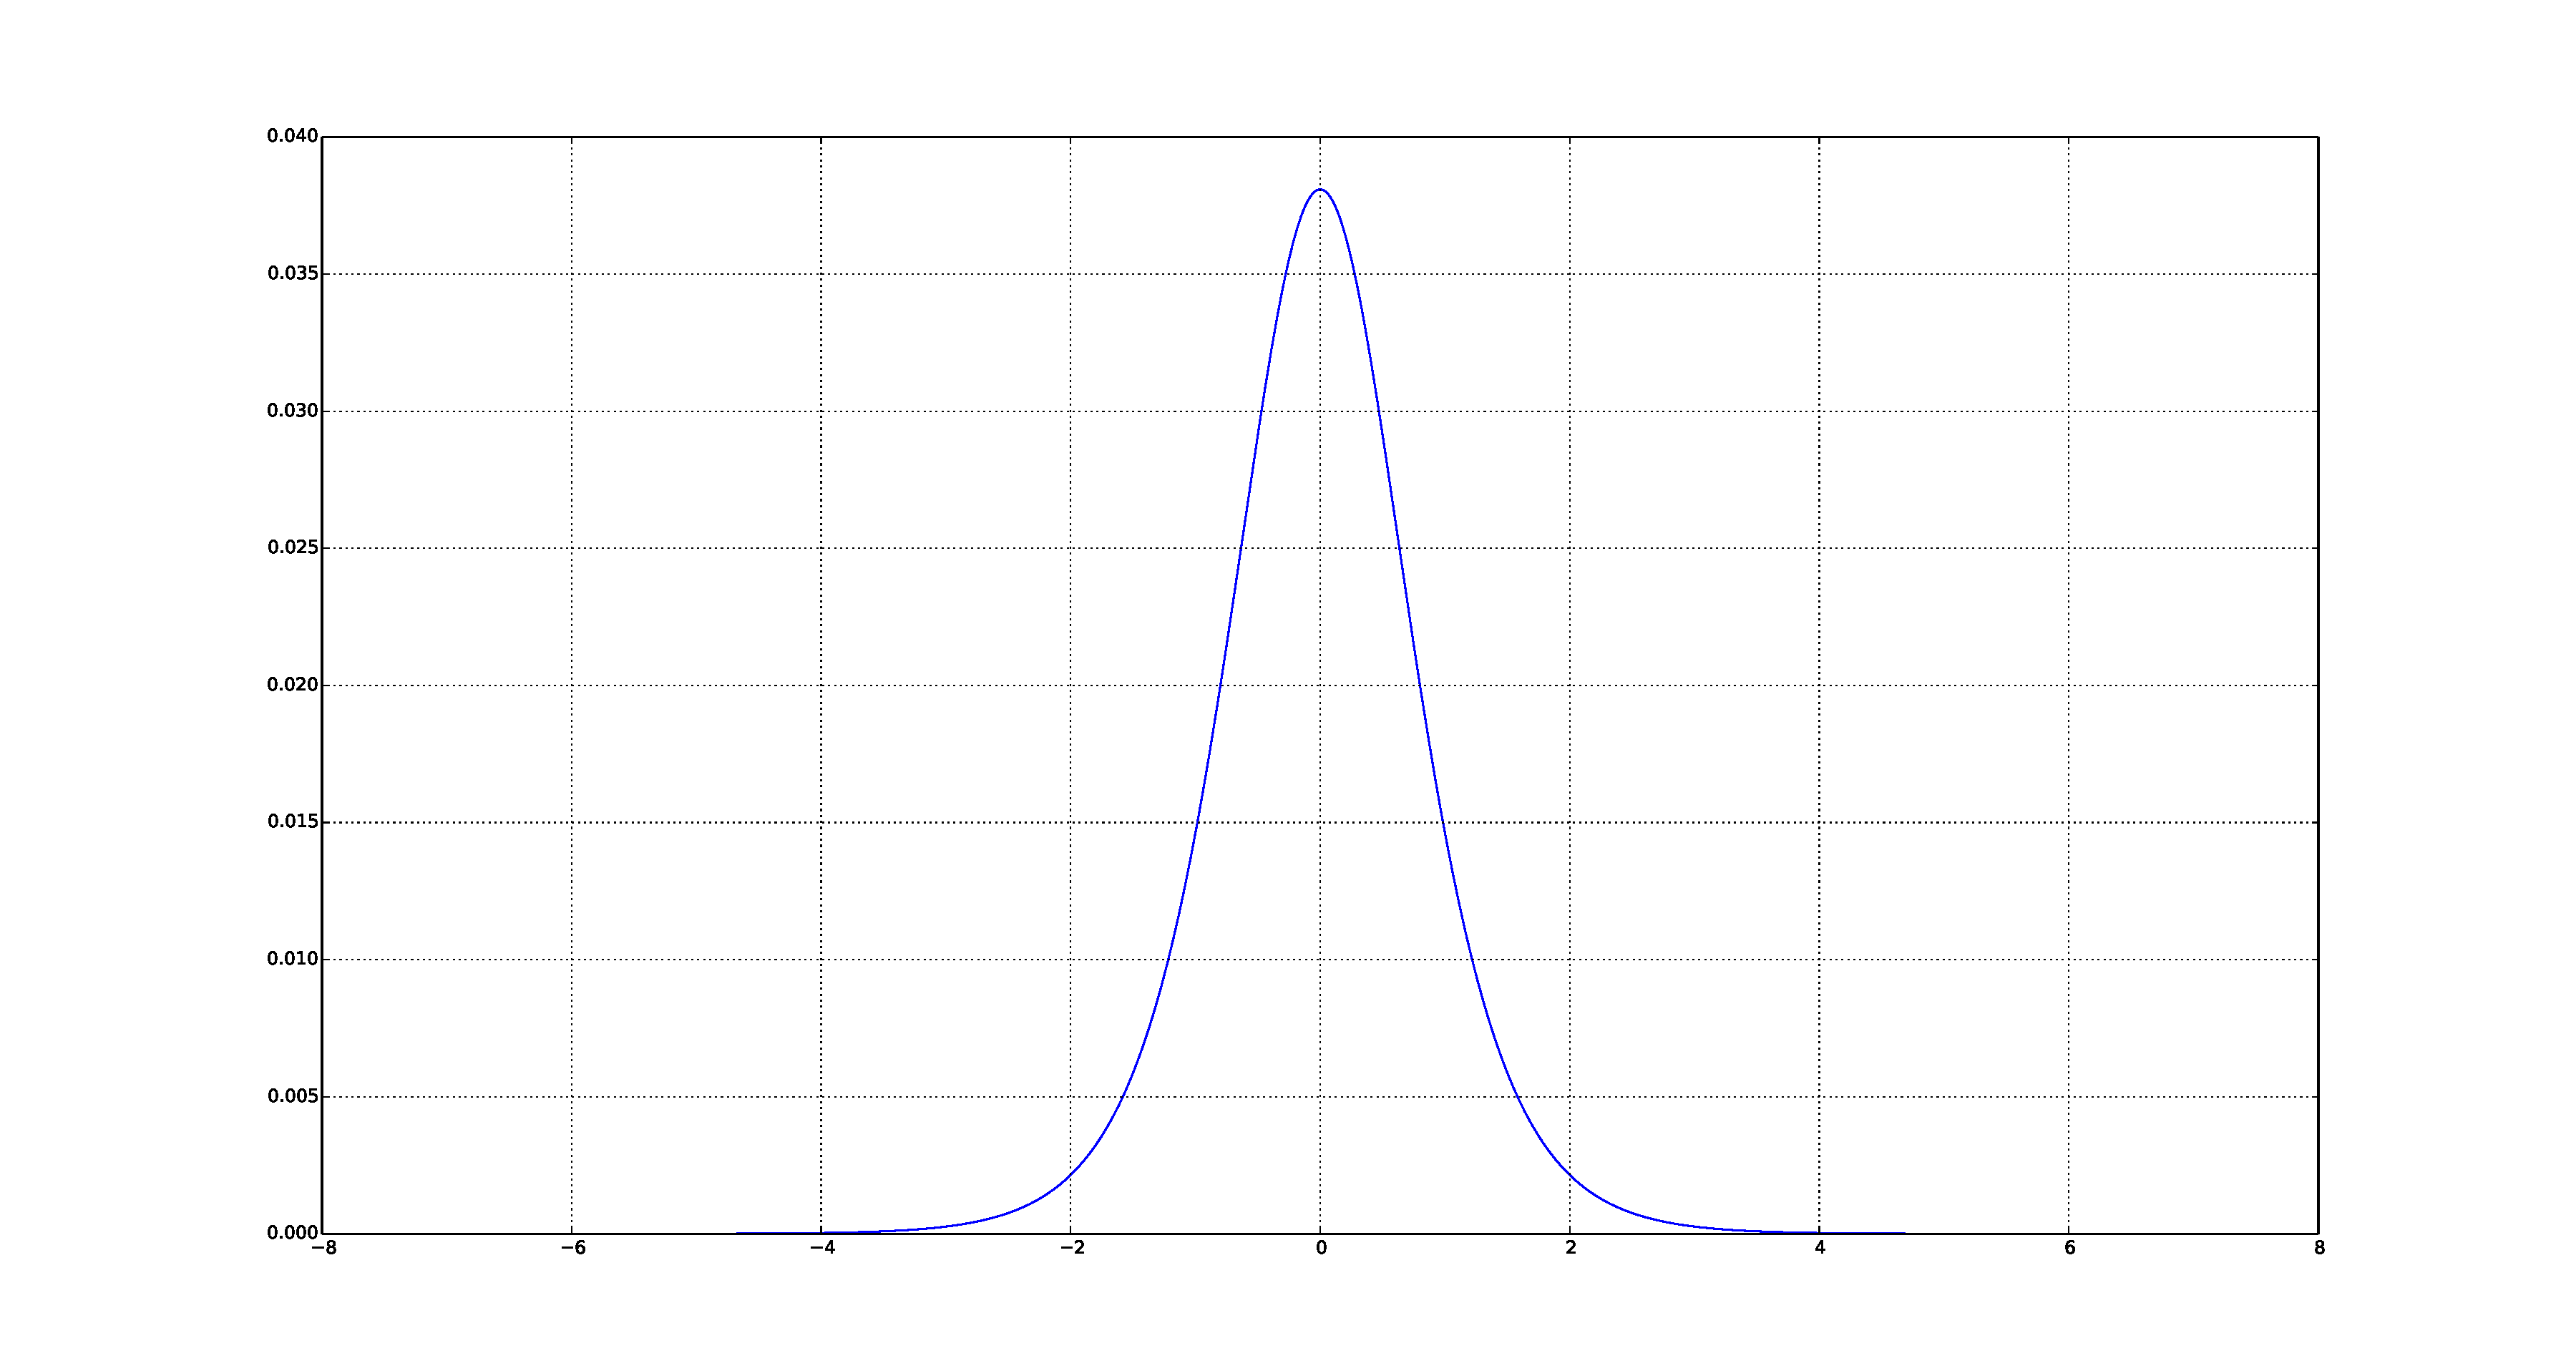
\includegraphics[width=\textwidth]{Figures/tunneling_pot.pdf}
\caption{Potential of the Tunneling Simulation}
\label{fig:tunneling_pot}
\end{figure}
\FloatBarrier

A Gaussian Hagedorn wavepacket with $512$ cubic shape basis functions with the following initial parameters:
\begin{center}
 \begin{tabular}{|c c c c c c|} 
 \hline
 q & p & Q & P & S & $\varepsilon$\\ [0.5ex] 
 \hline
 -7.5589045088306 & 0.2478854736792 & 3.5355339059327 & 0.2828427124746i & 0 & 0.02342\\ 
 \hline
\end{tabular}
\end{center}
is propagated using the Hagedorn propagator with $dt = 0.005$ up to $T = 70$.

\subsection{Observations}
Figures \ref{fig:tunneling_drift} and \ref{fig:tunneling_energy} show the potential and kinetic energies and the conservation of the total energy.
In Figure \ref{fig:tunneling_params} one can observe the packet being reflected at the origin and thus reversing its momentum.
The \texttt{C++} implementation appears to reproduce the data for Figure 1 in \cite{GHJ_tunneling_spawning} as evidenced by Figures \ref{fig:wavepacket_at_61_96}, \ref{fig:wavepacket_at_61_96} and \ref{fig:tunneling_coeffs_close}.  
Moreover, Figure \ref{fig:tunneling_coeffs} shows the increase in higher order coefficients when the packet gets closer to the origin which is responsible for the bump on right side of Figures \ref{fig:wavepacket_at_51_63} and \ref{fig:wavepacket_at_61_96}.
\begin{figure}
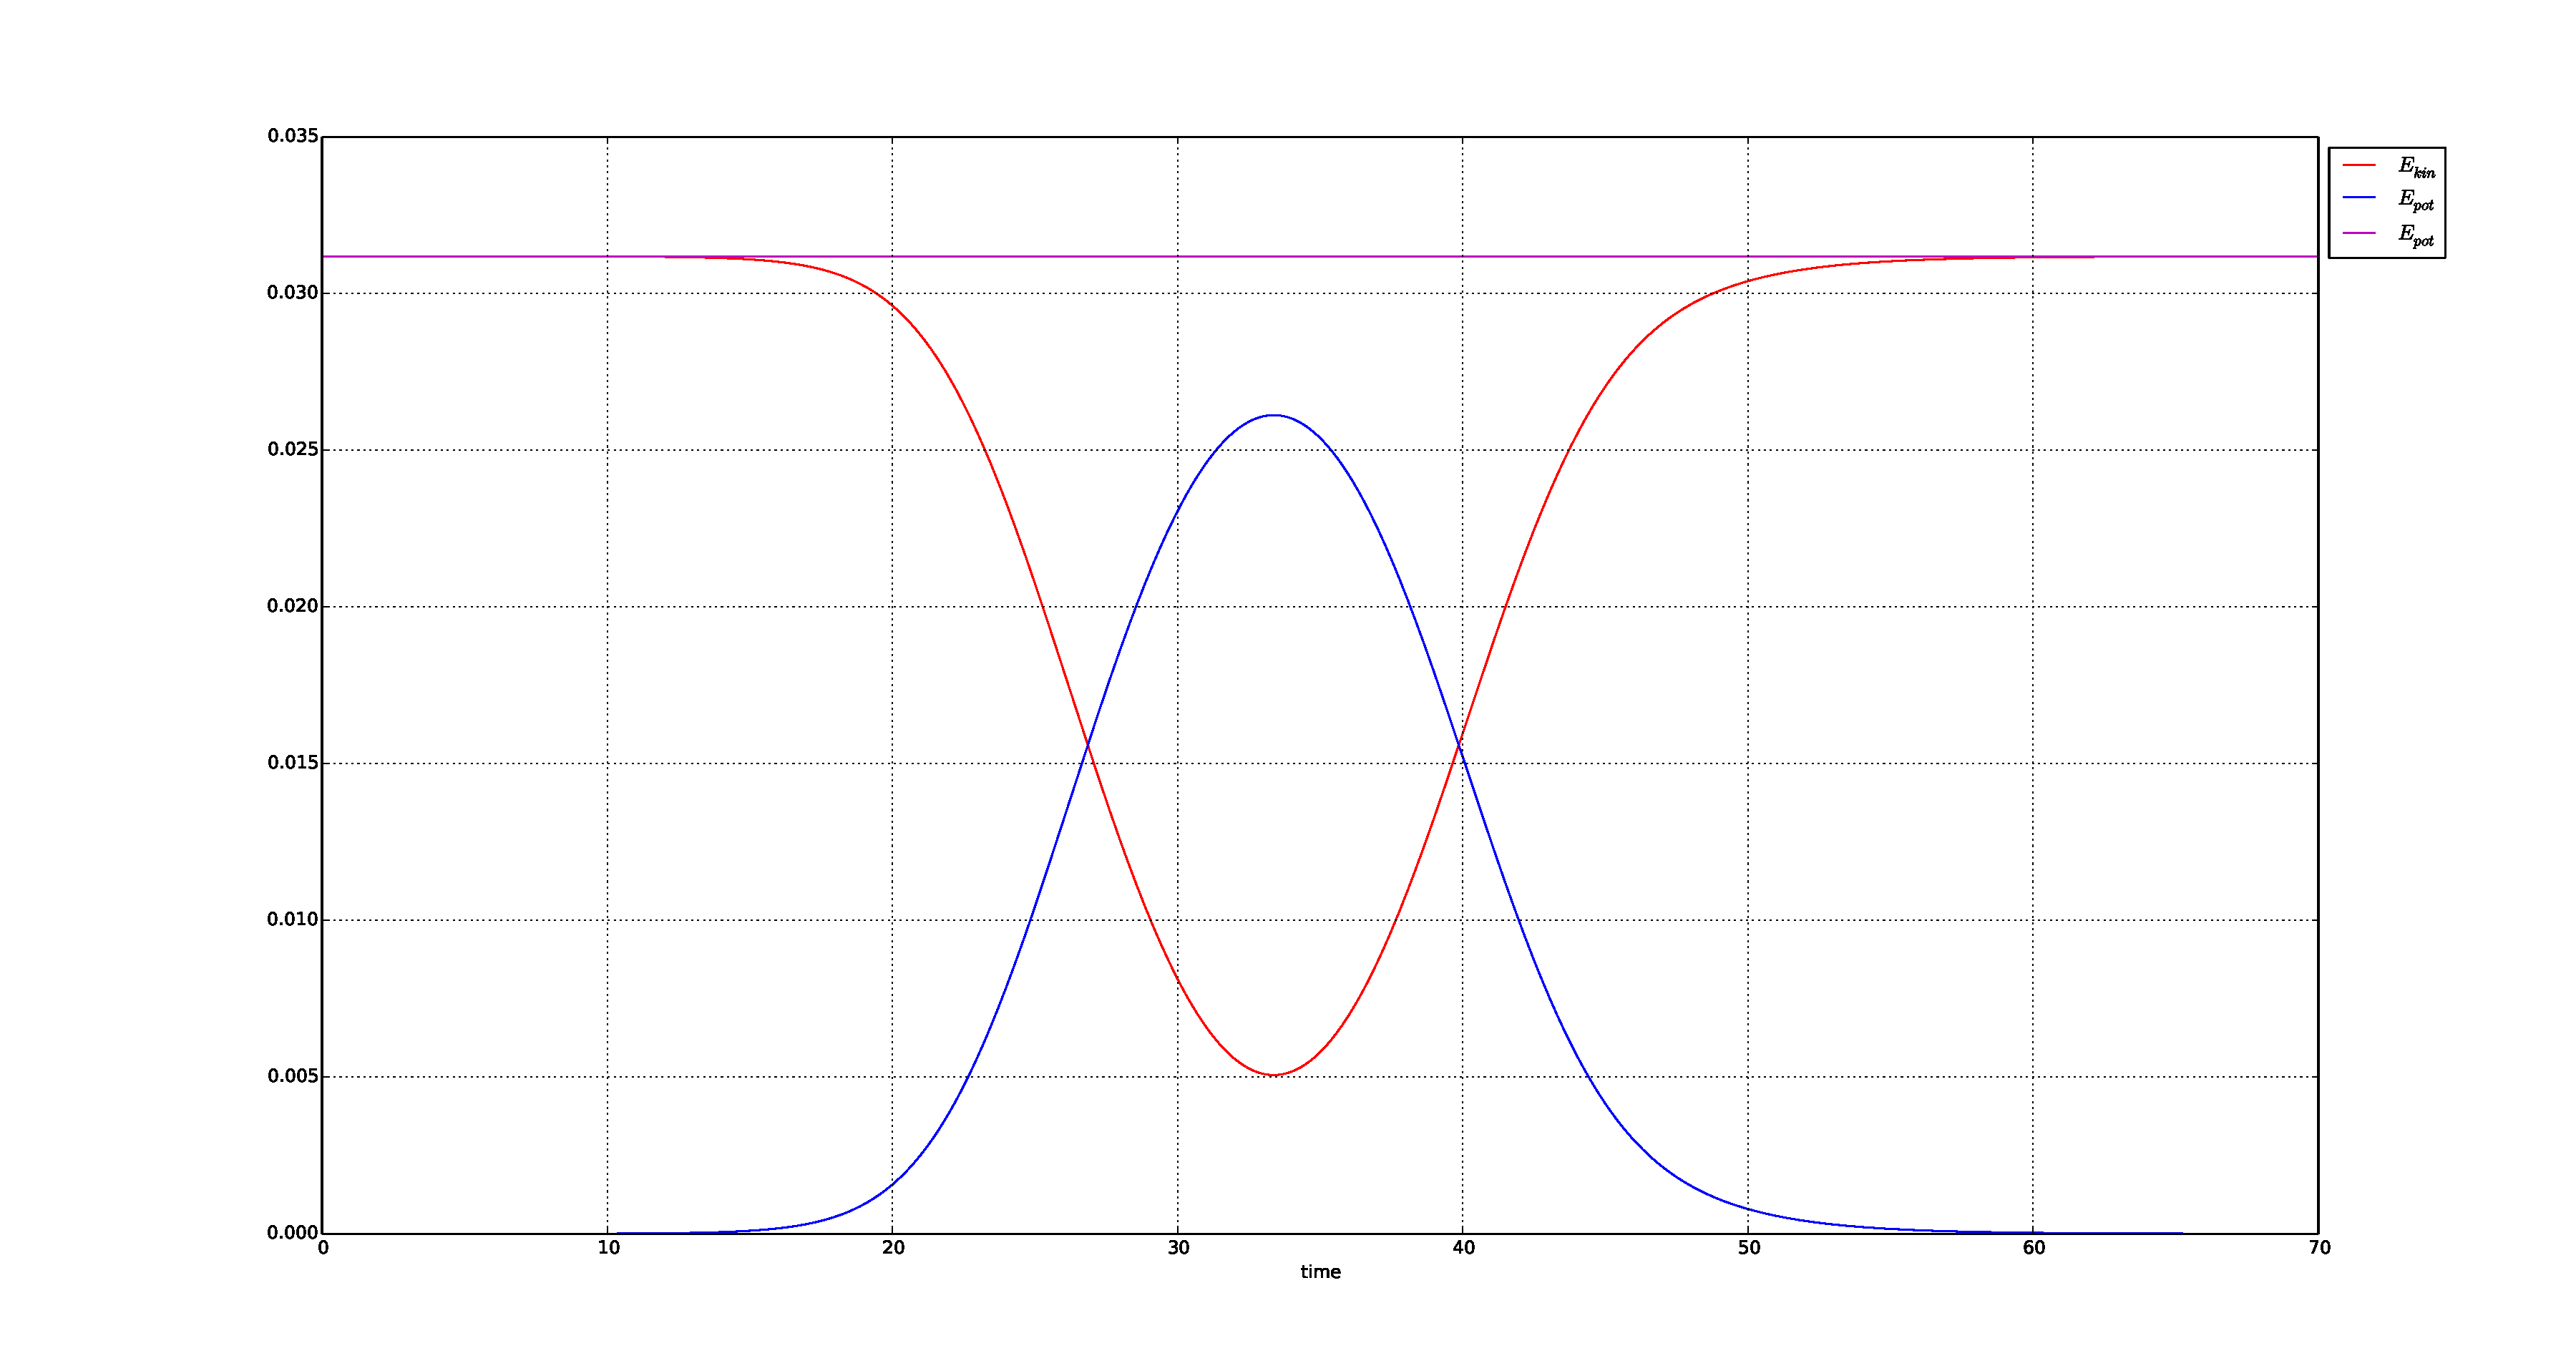
\includegraphics[width=\textwidth]{Figures/tunneling_energy.pdf}
\caption{Energies of the Tunneling Simulation}
\label{fig:tunneling_energy}
\end{figure}

\begin{figure}
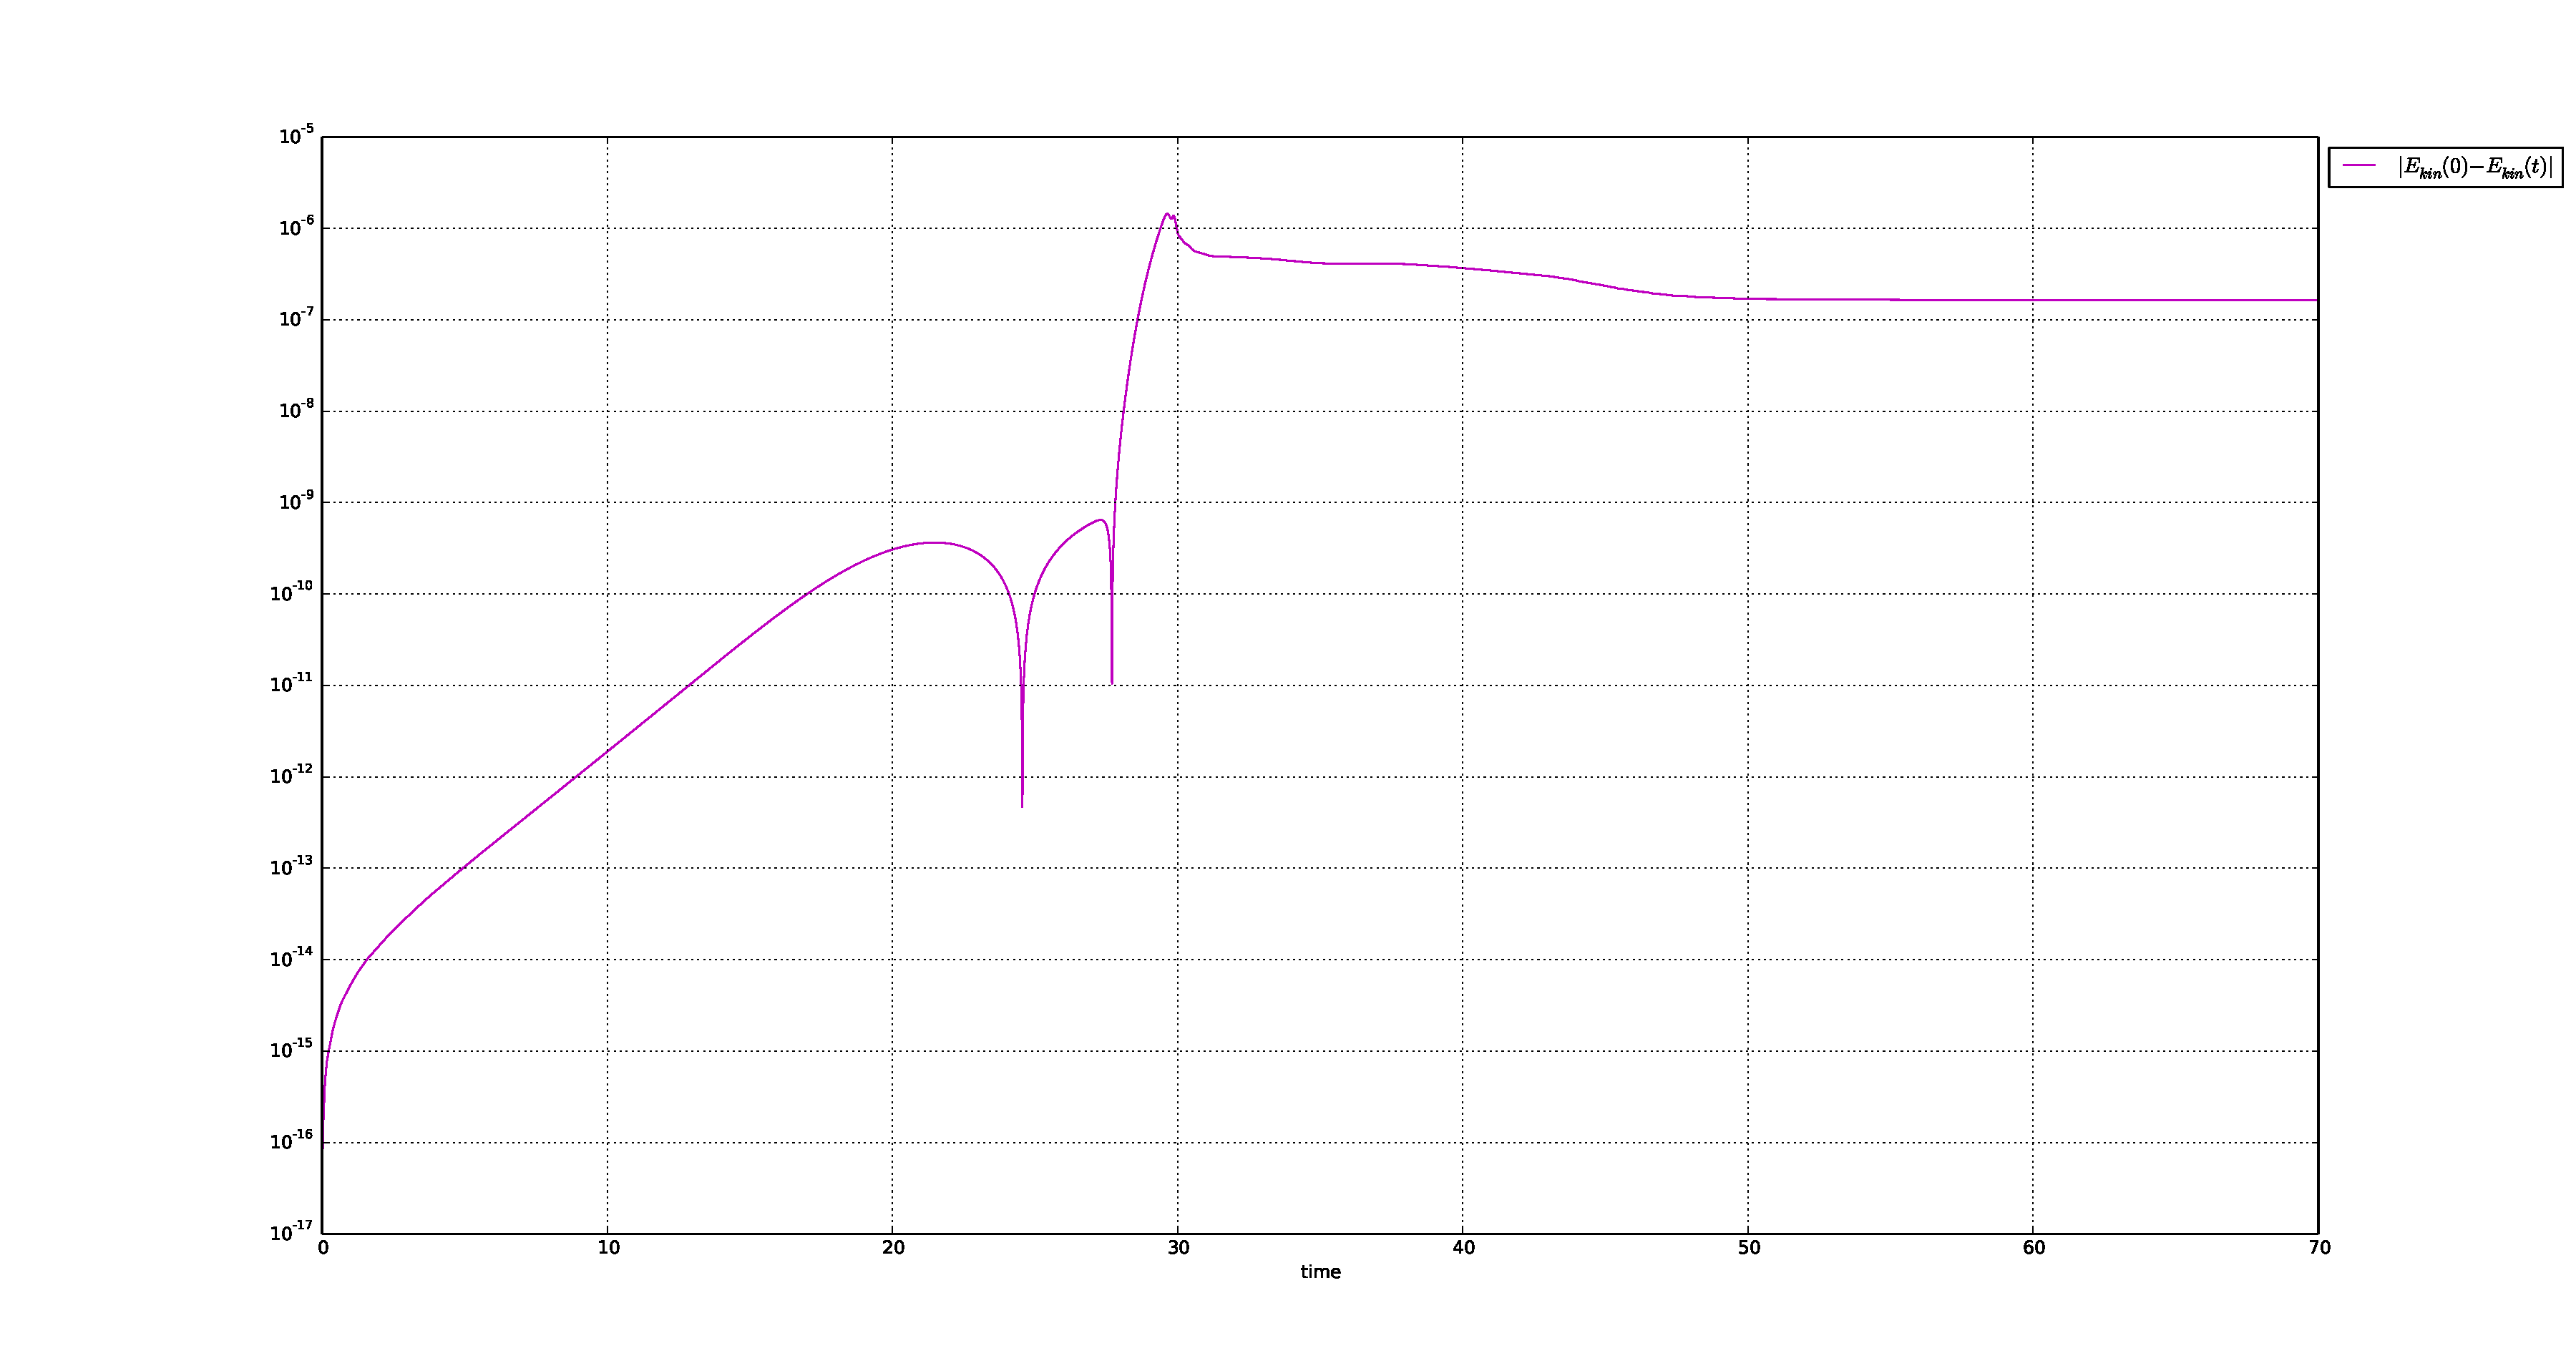
\includegraphics[width=\textwidth]{Figures/tunneling_drift.pdf}
\caption{Drift of Total Energy of the Tunneling Simulation}
\label{fig:tunneling_drift}
\end{figure} 	 	
\begin{figure}
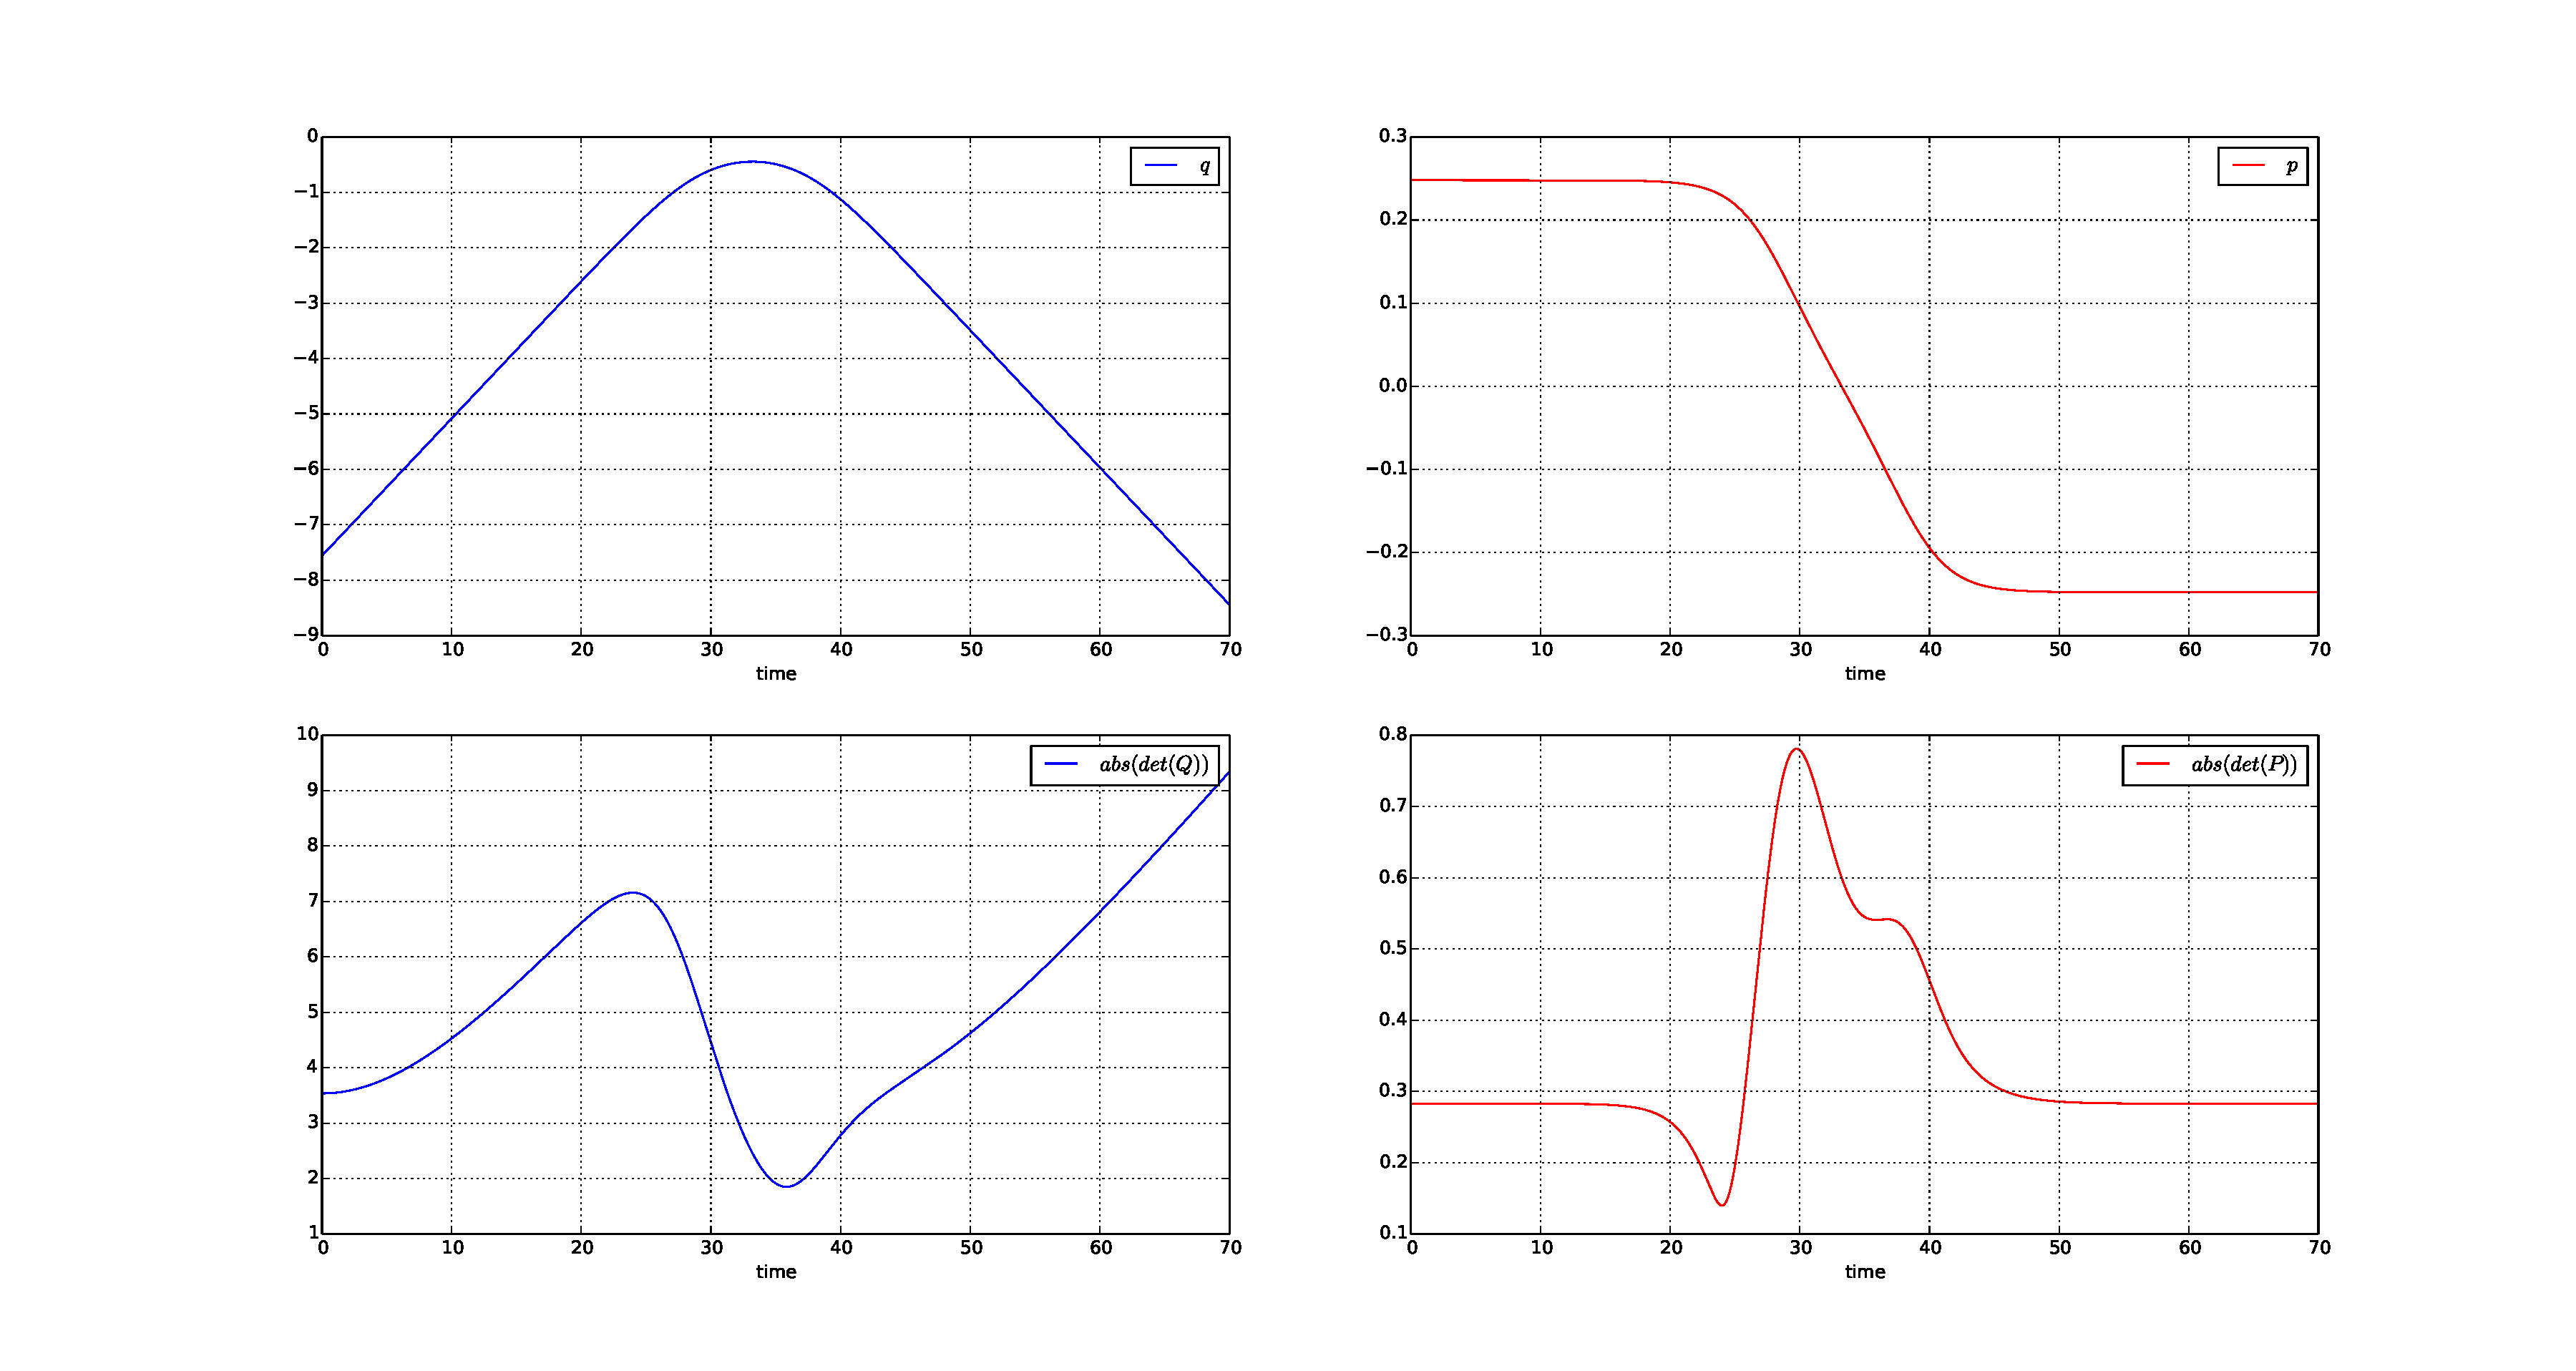
\includegraphics[width=\textwidth]{Figures/tunneling_params.pdf}
\caption{Position and Momentum Parameters}
\label{fig:tunneling_params}
\end{figure}
\begin{figure}
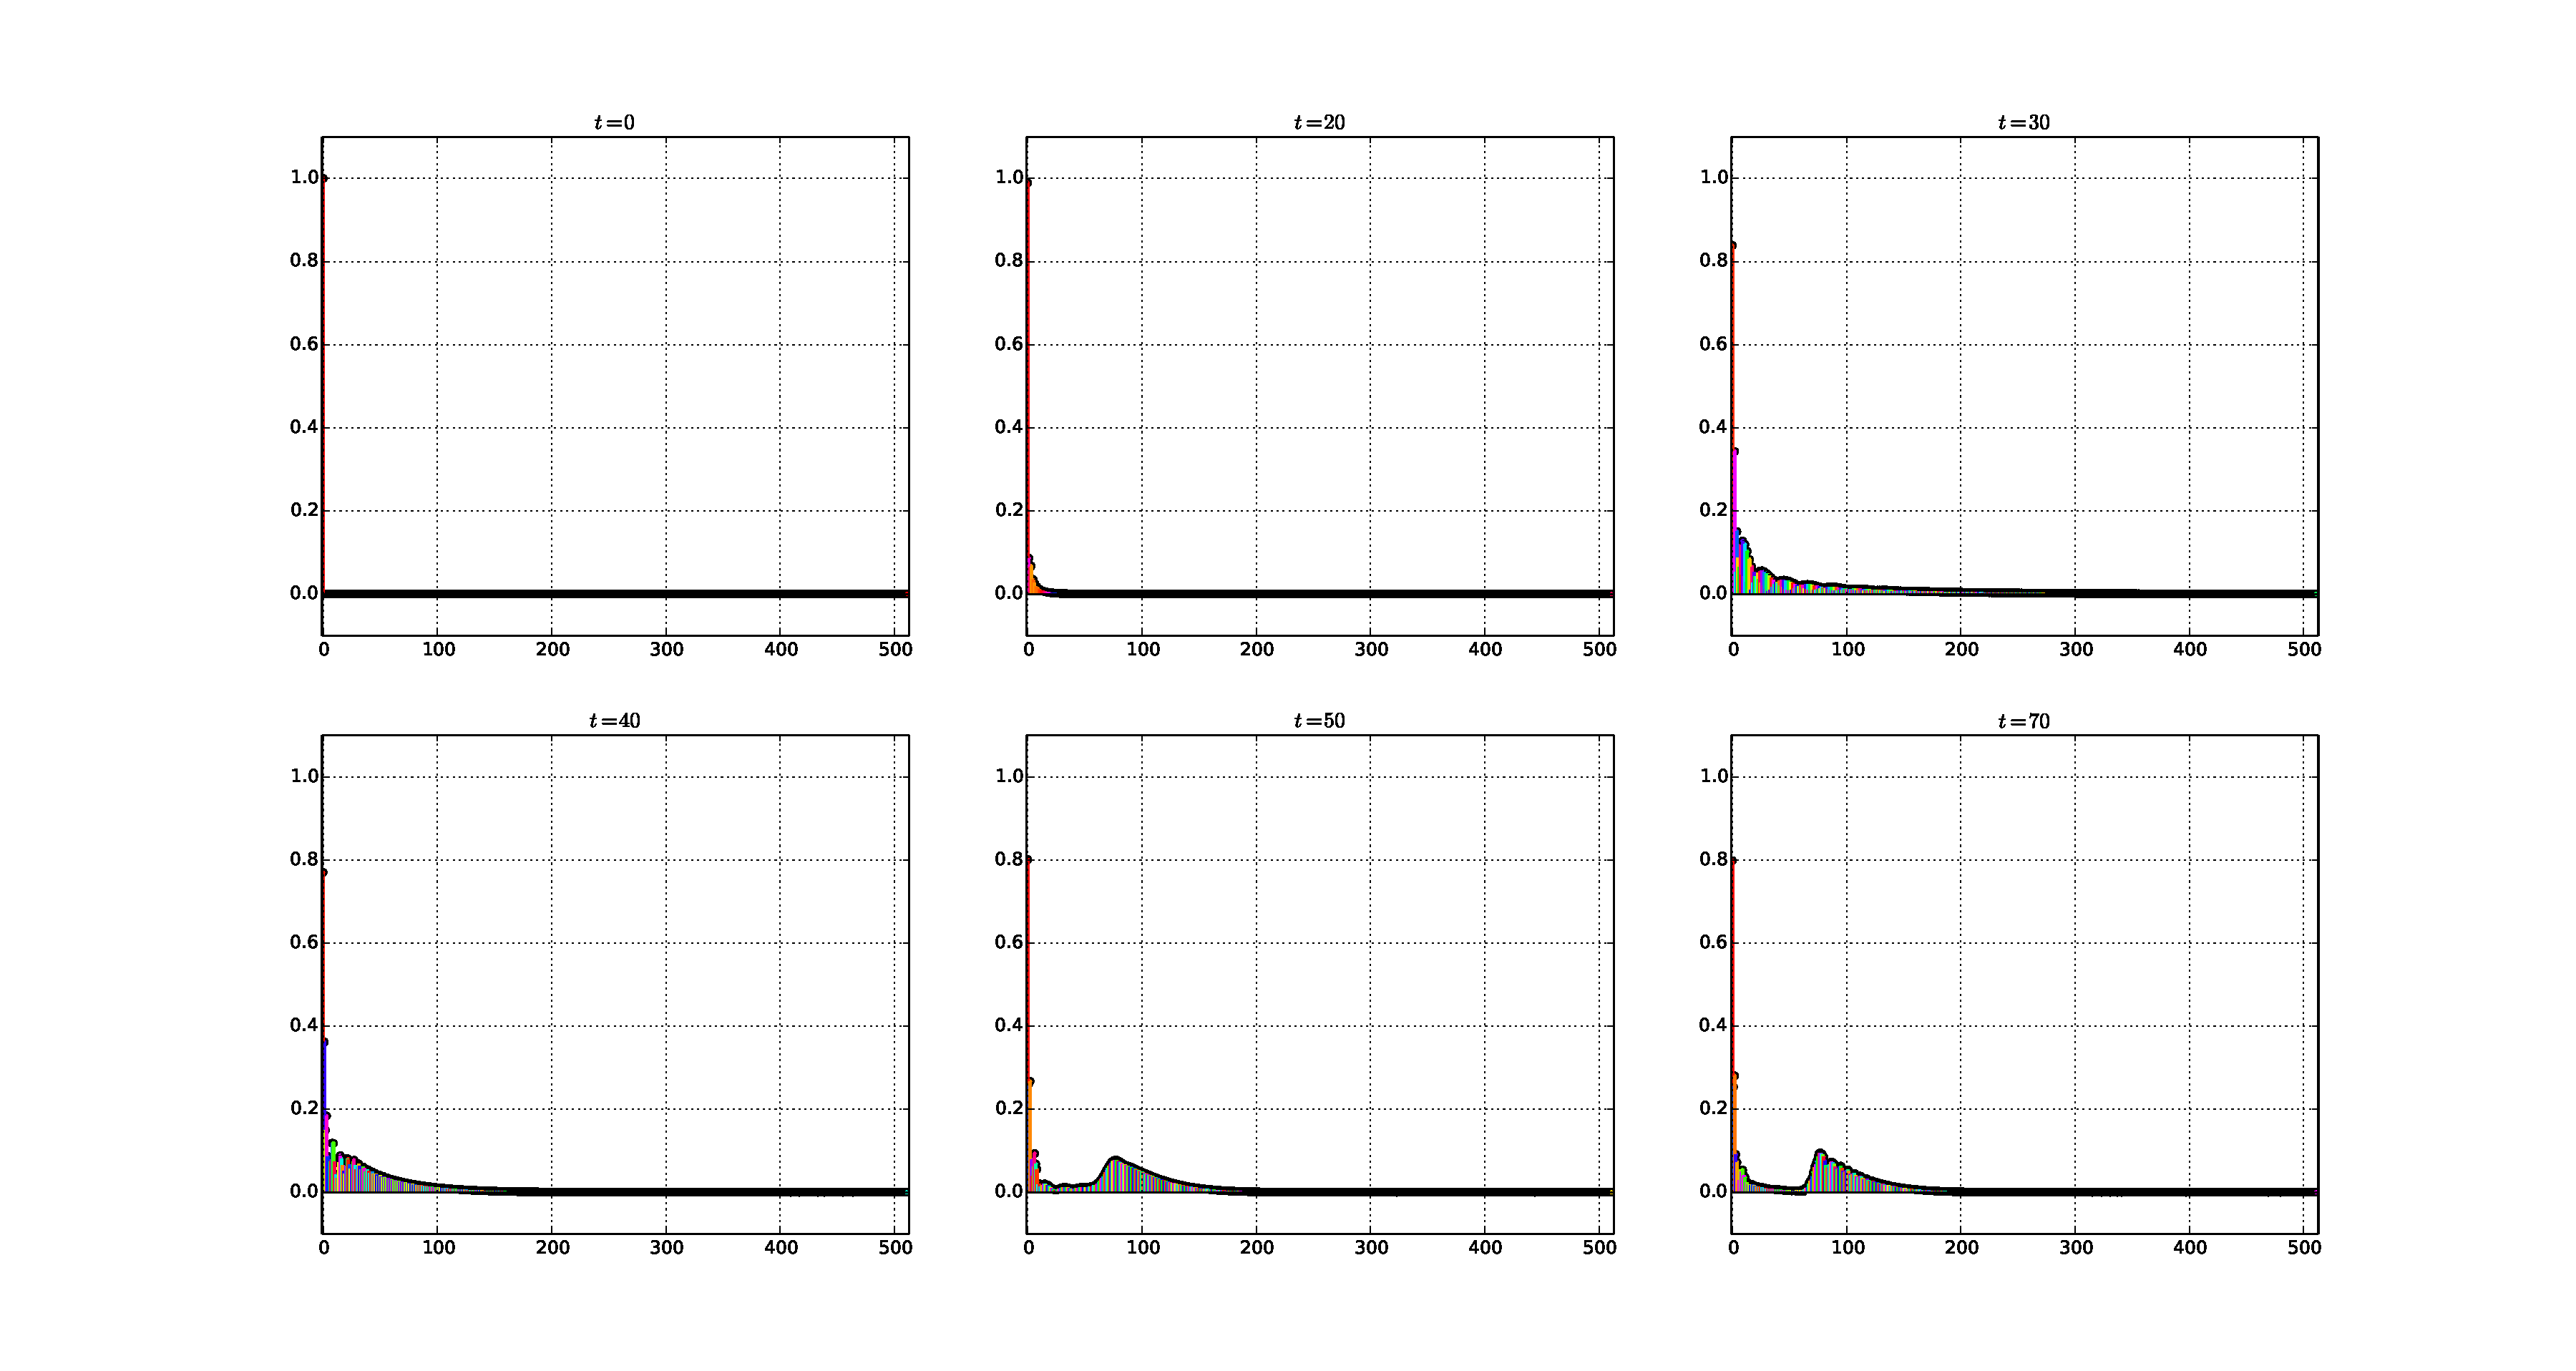
\includegraphics[width=\textwidth]{Figures/tunneling_coeffs.pdf}
\caption{Coefficients}
\label{fig:tunneling_coeffs}
\end{figure}

\begin{figure}
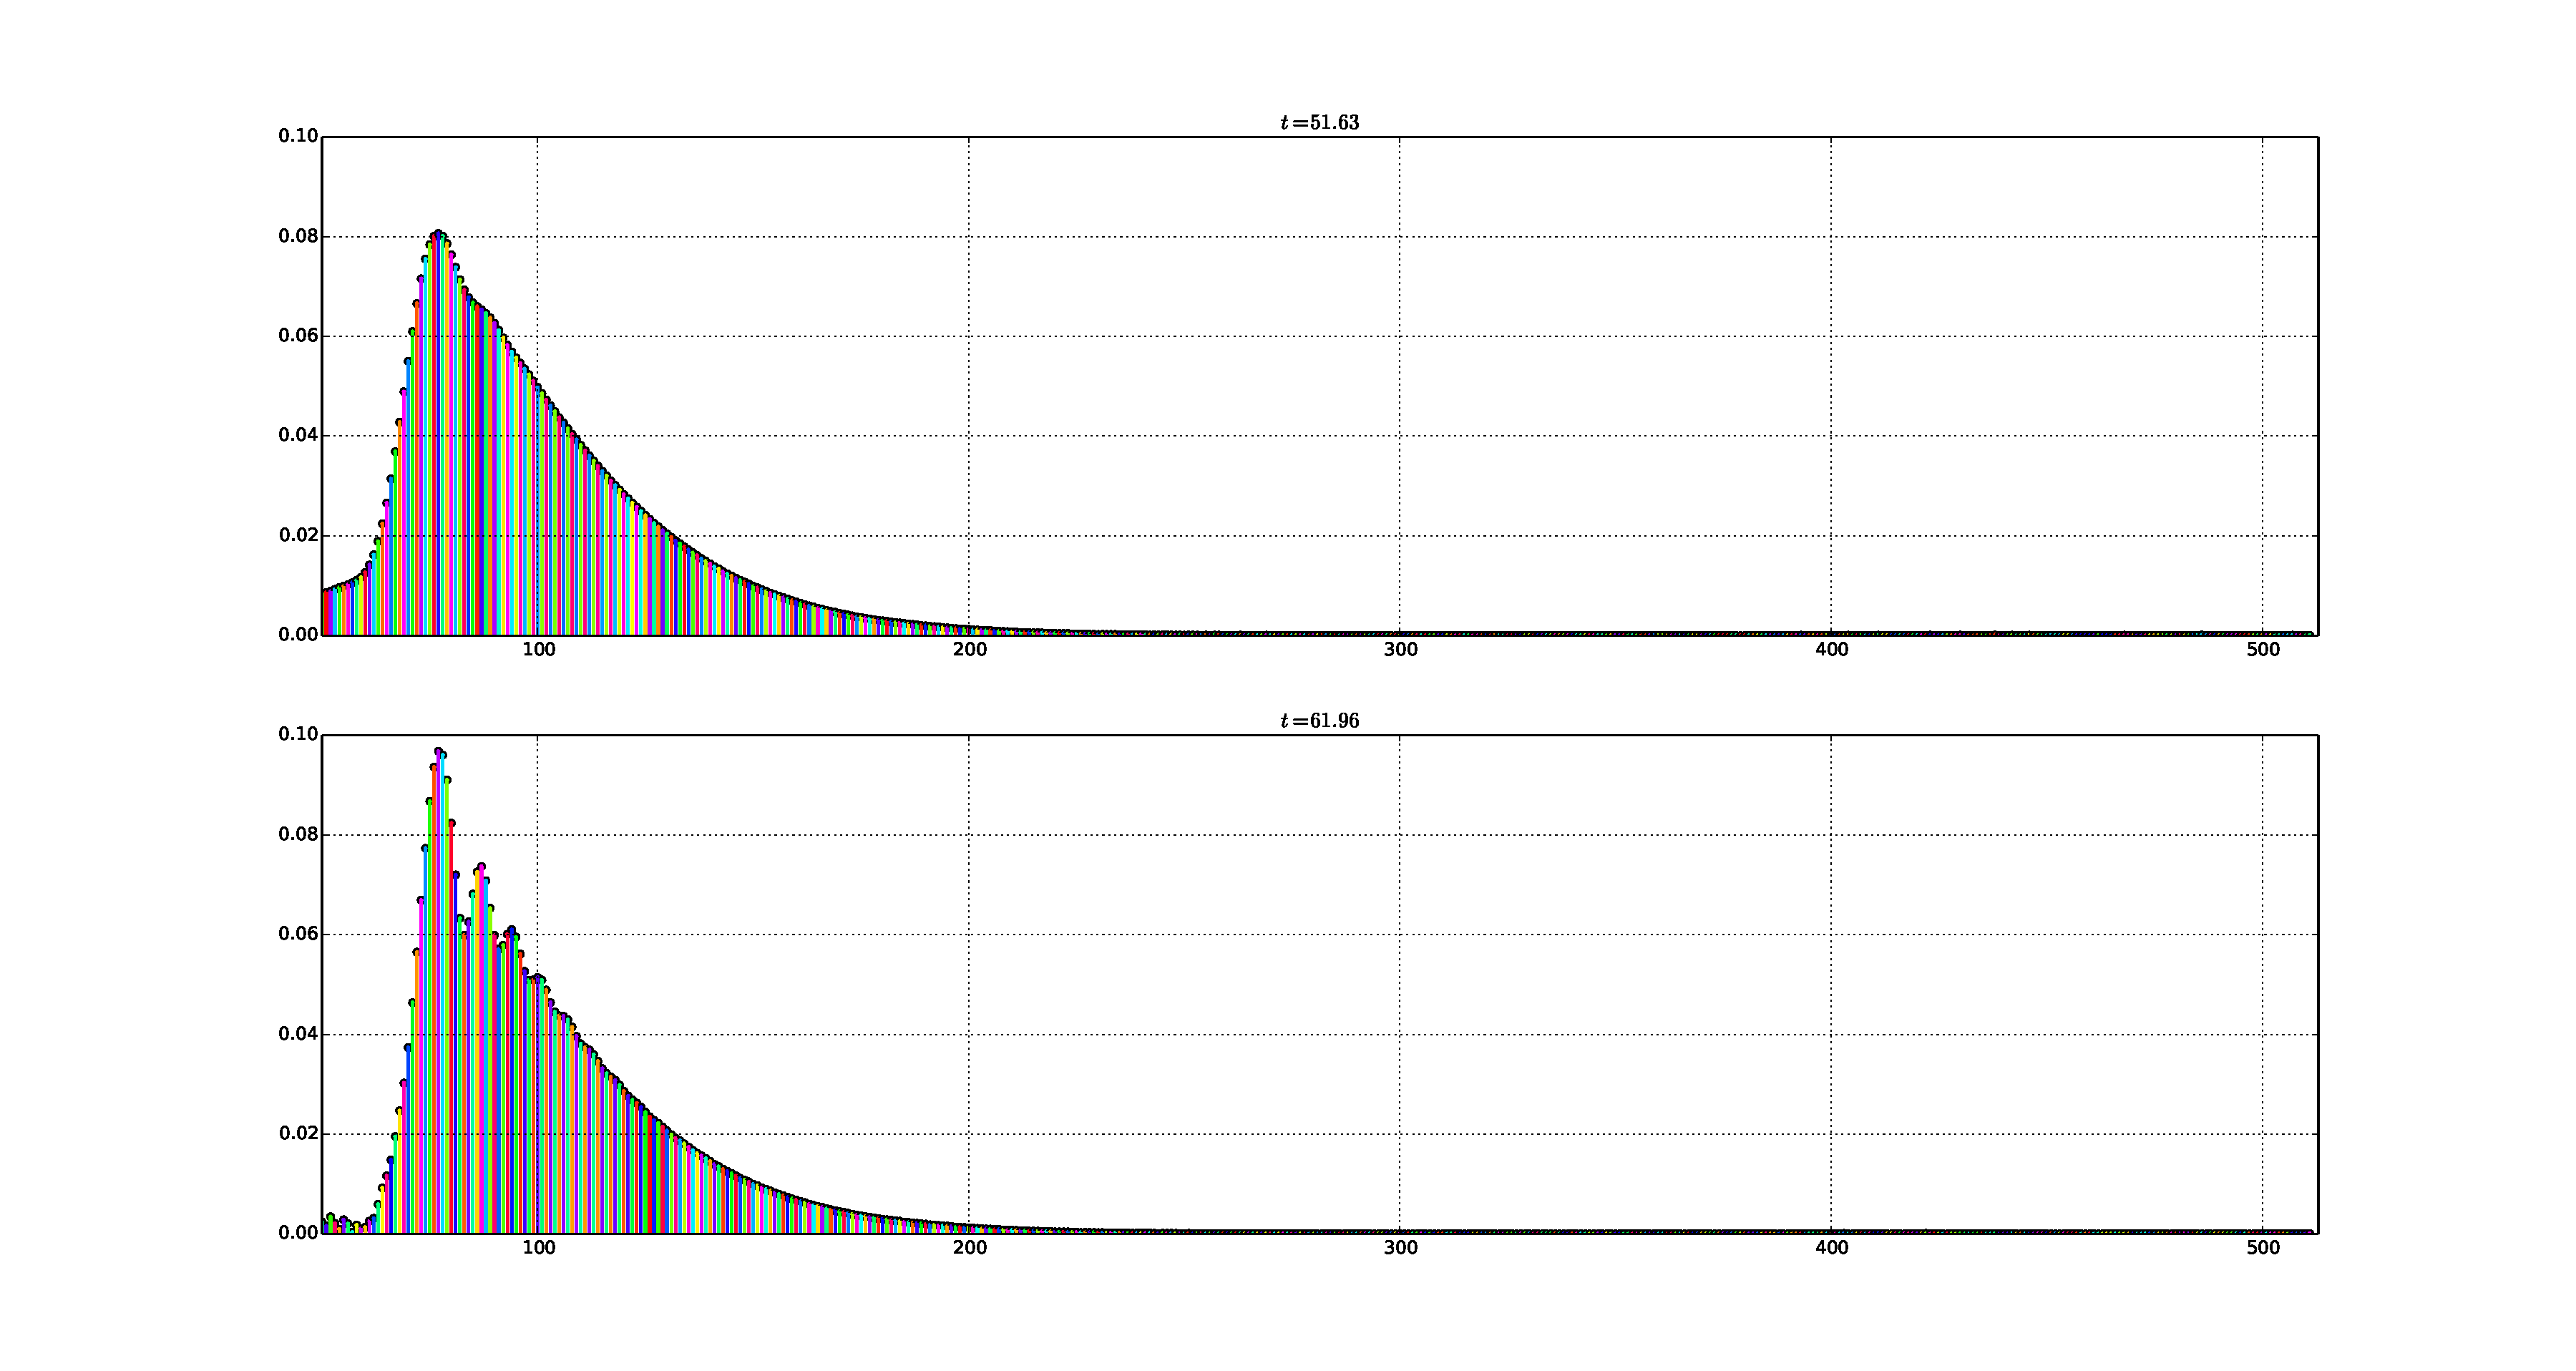
\includegraphics[width=\textwidth]{Figures/tunneling_coeffs_close.pdf}
\caption{close-up of Higher Order Coefficients}
\label{fig:tunneling_coeffs_close}
\end{figure}

\begin{figure}
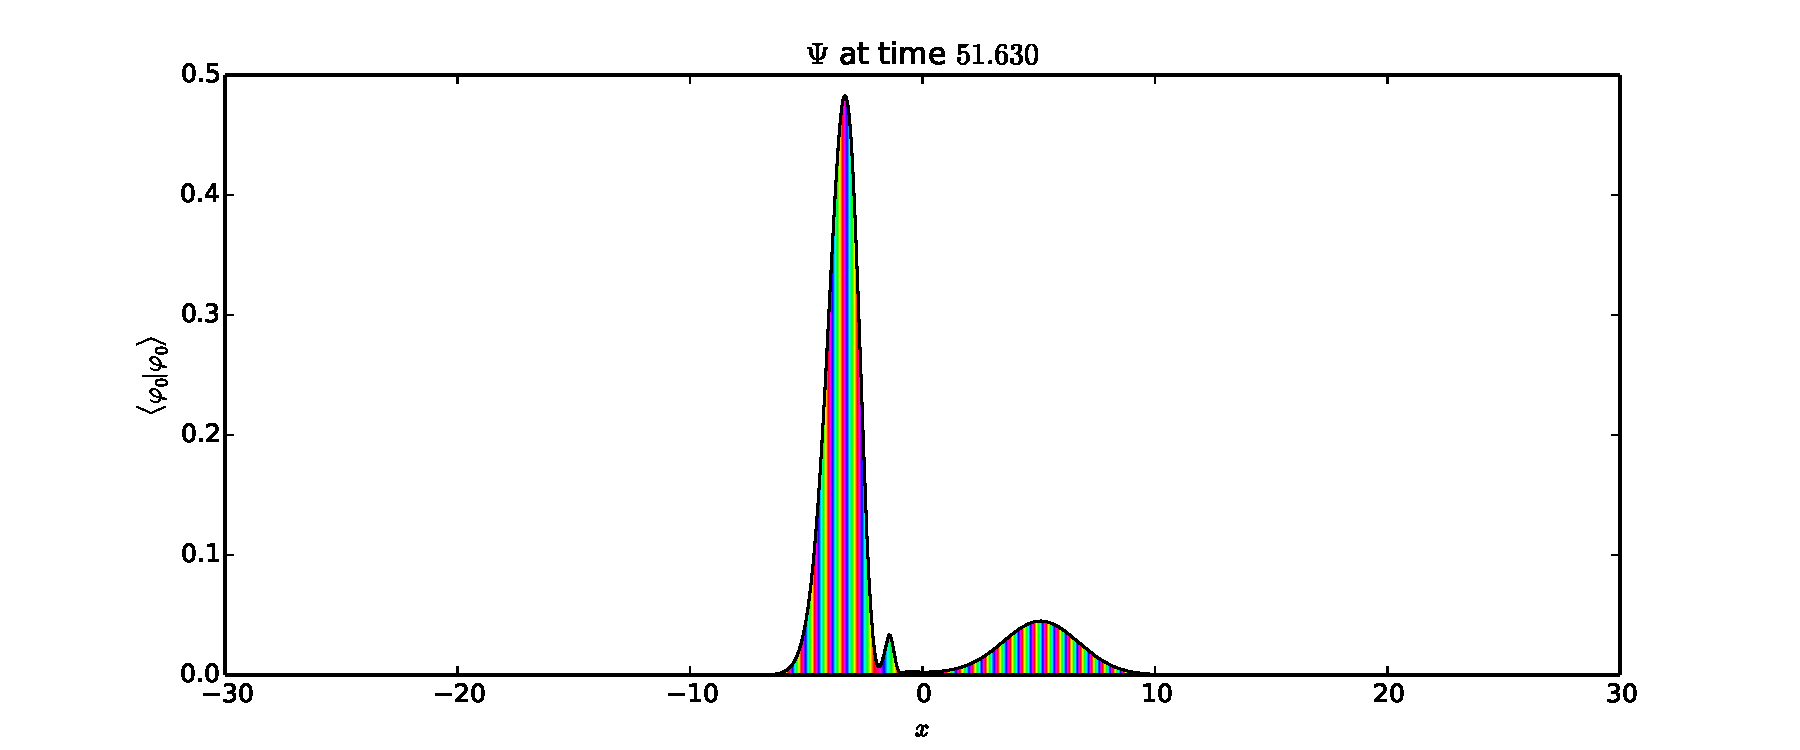
\includegraphics[width=\textwidth]{Figures/wavepacket_timestep_51_630.pdf}
\caption{$|u^2|$ at $t=51.63$}
\label{fig:wavepacket_at_51_63}
\end{figure}

\begin{figure}
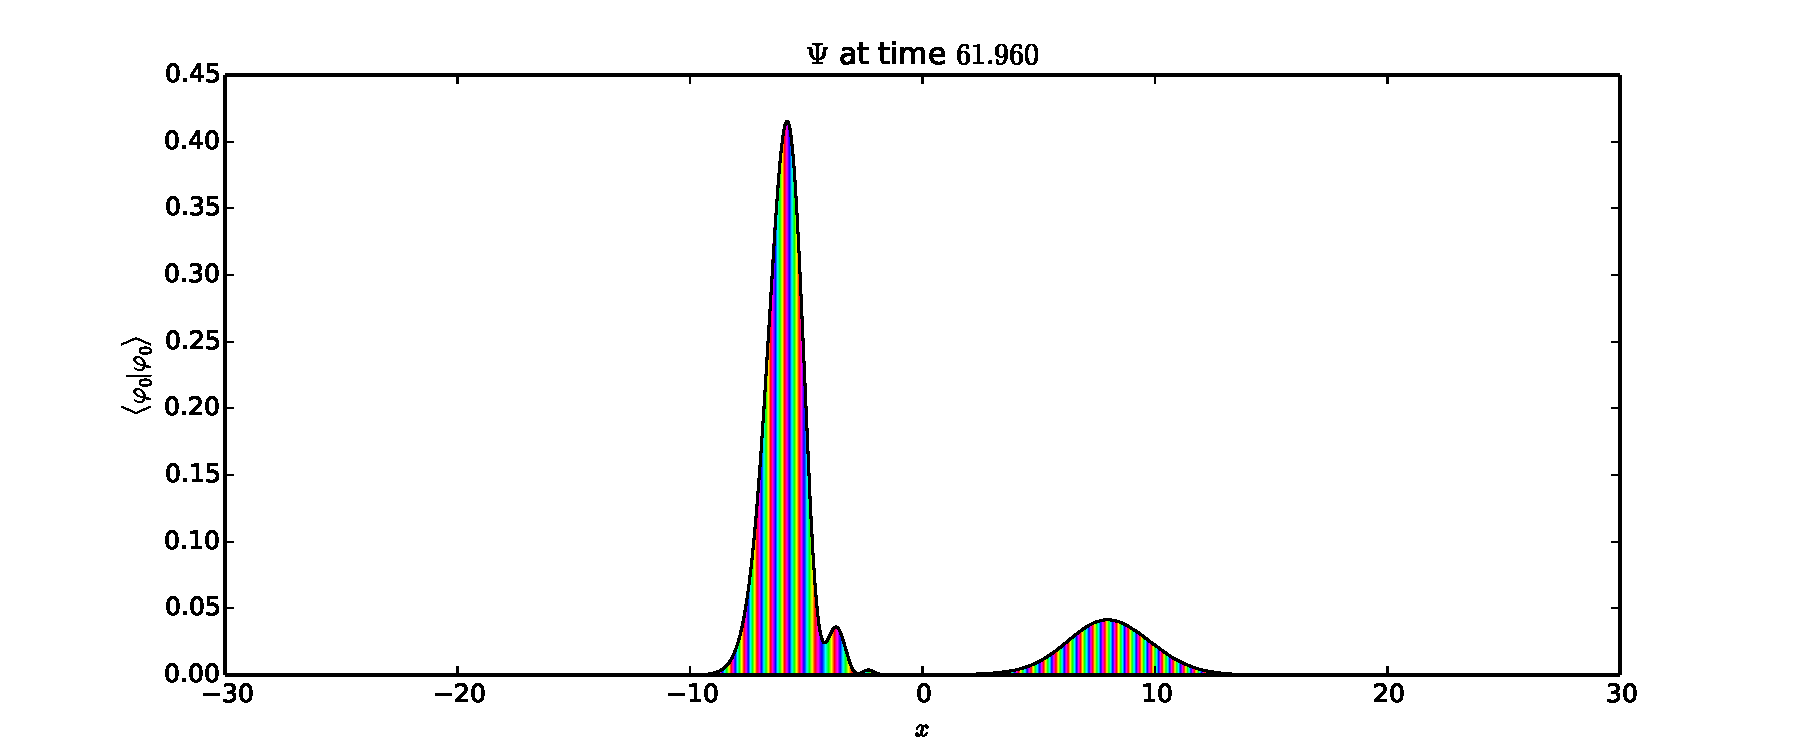
\includegraphics[width=\textwidth]{Figures/wavepacket_timestep_61_960.pdf}
\caption{$|u^2|$ at $t=61.96$}
\label{fig:wavepacket_at_61_96}
\end{figure}
\FloatBarrier
 
%\input{./Chapters/Chapter6} 
%\input{./Chapters/Chapter7} 

\addtocontents{toc}{\vspace{2em}} % Add a gap in the Contents, for aesthetics

\backmatter


%----------------------------------------------------------------------------------------
%	BIBLIOGRAPHY
%----------------------------------------------------------------------------------------

\label{Bibliography}

\lhead{\emph{References}} % Change the page header to say "Bibliography"

\bibliographystyle{plain}
\bibliography{Bibliography} % The references (bibliography) information are stored in the file named "Bibliography.bib"

\end{document}